% =============================================================================
% kMC 3D de crecimiento cristalino (3DkMC/kmc3d): fundamentos teóricos, modelo,
% algoritmo e implementación.
%
% Compilación (XeLaTeX vía tectonic), desde 3DkMC/teoria/:
%     tectonic teoria_3DkMC.tex
% Figuras de datos (las calcula el propio kmc3d) y copia de las del notebook 01:
%     python 3DkMC/teoria/make_figures.py
% Los diagramas conceptuales están en TikZ dentro de este archivo.
% =============================================================================
\documentclass[11pt,a4paper]{article}

% ---------------------------------------------------------------- tipografía
\usepackage{fontspec}
\usepackage{unicode-math}
% TeX Gyre Pagella por nombre de archivo (igual que explainer/slides_observables.tex)
\setmainfont{texgyrepagella}[Extension=.otf, UprightFont=*-regular, BoldFont=*-bold,
  ItalicFont=*-italic, BoldItalicFont=*-bolditalic]
\setmonofont{lmmono10-regular.otf}[Scale=0.95]
\setmathfont{texgyrepagella-math.otf}
\usepackage[spanish,es-noshorthands,es-nodecimaldot,es-tabla]{babel}

% ---------------------------------------------------------------- paquetes
\usepackage[a4paper,margin=2.2cm,top=2.0cm,bottom=2.2cm]{geometry}
\usepackage{amsmath,mathtools}
\usepackage{booktabs,array,tabularx,multirow}
\usepackage{graphicx}
\usepackage{xcolor}
\usepackage{tikz}
\usetikzlibrary{arrows.meta,positioning,calc,decorations.pathreplacing,fit,backgrounds,
  shapes.misc,shapes.geometric}
\usepackage[most]{tcolorbox}
\usepackage{algorithm}
\usepackage{algpseudocode}
\usepackage[font=small,labelfont=bf,labelsep=period]{caption}
\usepackage{subcaption}
\usepackage{enumitem}
\usepackage{float}
\usepackage[section]{placeins}
\usepackage[colorlinks=true,linkcolor=navy,citecolor=teal,urlcolor=azul]{hyperref}

\setlist{itemsep=1pt,topsep=3pt,parsep=0pt}
\setlength{\parskip}{3pt}
\setlength{\emergencystretch}{3em}
\makeatletter\setlength{\@fptop}{0pt}\setlength{\@fpsep}{14pt plus 4pt}\makeatother
\newcolumntype{Y}{>{\raggedright\arraybackslash}X}
\graphicspath{{figuras/}}

% ---------------------------------------------------------------- colores
\definecolor{navy}{HTML}{0D366B}
\definecolor{azul}{HTML}{0072BD}
\definecolor{teal}{HTML}{2B8A96}
\definecolor{carmin}{HTML}{A2142F}
\definecolor{naranja}{HTML}{D95319}
\definecolor{amarillo}{HTML}{EDB120}
\definecolor{verde}{HTML}{77AC30}
\definecolor{morado}{HTML}{7E2F8E}
\definecolor{gris}{HTML}{52514E}
\definecolor{grisclaro}{HTML}{F0EFEC}

% ---------------------------------------------------------------- cajas
% Supuestos del modelo (numerados S1, S2, ... a mano, para citarlos en el texto)
\newtcolorbox{supuesto}[1]{enhanced,breakable,colback=grisclaro,colframe=navy,
  boxrule=0.4pt,arc=1.5pt,left=5pt,right=5pt,top=2pt,bottom=2pt,
  fonttitle=\bfseries\small,coltitle=white,title={#1},before skip=5pt,after skip=5pt}
% Observaciones técnicas (lo que hay que saber de la implementación)
\newtcolorbox{nota}[1]{enhanced,breakable,colback=white,colframe=carmin,
  boxrule=0.4pt,arc=1.5pt,left=5pt,right=5pt,top=2pt,bottom=2pt,
  fonttitle=\bfseries\small,coltitle=white,title={#1},before skip=5pt,after skip=5pt}

% ---------------------------------------------------------------- algoritmos en español
\floatname{algorithm}{Algoritmo}
\algrenewcommand\algorithmicif{\textbf{si}}
\algrenewcommand\algorithmicthen{\textbf{entonces}}
\algrenewcommand\algorithmicelse{\textbf{si no}}
\algrenewcommand\algorithmicfor{\textbf{para}}
\algrenewcommand\algorithmicdo{\textbf{hacer}}
\algrenewcommand\algorithmicwhile{\textbf{mientras}}
\algrenewcommand\algorithmicreturn{\textbf{devolver}}
\algrenewcommand\algorithmicend{\textbf{fin}}
\algrenewcommand\algorithmicfunction{\textbf{función}}
\algrenewcommand\algorithmicprocedure{\textbf{procedimiento}}

% ---------------------------------------------------------------- macros
\newcommand{\code}[1]{\texttt{#1}}
\newcommand{\vect}[1]{\mathbf{#1}}
\newcommand{\Ekink}{E_{\mathrm{kink}}}
\newcommand{\Ecr}{E_{\mathrm{cr}}}
\newcommand{\Eslice}{E_{\mathrm{slice}}}
\newcommand{\Eatt}{E_{\mathrm{att}}}
\newcommand{\dmu}{\Delta\mu}
\newcommand{\bh}{$\beta$-hematina}
\newcommand{\hkl}[1]{$(#1)$}

% ---------------------------------------------------------------- cubo isométrico (TikZ)
% \cubo{x}{y}{z}{color}: cara frontal (y = cte), superior (+z) y lateral derecha (+x)
\newcommand{\cubo}[4]{%
  \filldraw[fill=#4!28,draw=black!75,line width=0.25pt] (#1,#2,#3) -- ++(1,0,0) -- ++(0,0,1) -- ++(-1,0,0) -- cycle;
  \filldraw[fill=#4!10,draw=black!75,line width=0.25pt] (#1,#2,{#3+1}) -- ++(1,0,0) -- ++(0,1,0) -- ++(-1,0,0) -- cycle;
  \filldraw[fill=#4!50,draw=black!75,line width=0.25pt] ({#1+1},#2,#3) -- ++(0,1,0) -- ++(0,0,1) -- ++(0,-1,0) -- cycle;}

\title{\vspace{-0.6cm}\textbf{Modelo kMC tridimensional de crecimiento cristalino}\\[2pt]
\large Fundamentos teóricos, ecuaciones, supuestos e implementación del paquete \code{3DkMC/kmc3d}}
\author{Proyecto \code{kMC\_Malaria} --- documento técnico}
\date{9 de noviembre de 2026}

\begin{document}
\maketitle
\vspace{-0.5cm}

\begin{abstract}
\noindent Este documento describe en detalle el motor \emph{kinetic Monte Carlo} tridimensional
\code{3DkMC}: un cristal \emph{finito} que crece o se disuelve por \emph{todas} sus caras a la vez,
sobre una red de Bravais arbitraria (triclínica incluida) con una unidad de crecimiento por
celda. La anisotropía no se impone a mano: sale de un \emph{grafo de enlaces} (un vector de red
y una energía por tipo de enlace), del que se deducen también las energías de capa y de unión de
Hartman--Perdok y el carácter F/S/K de cada cara. Se exponen la geometría cristalina, la energética,
la termodinámica de las tasas (con su equivalencia exacta con un gas de red), el algoritmo BKL
(\emph{n-fold way}) incremental con árbol de Fenwick, la gestión de la caja, los observables por
cara y de forma (Wulff cinético), la validación (47 tests) y los primeros resultados en Kossel,
cubitos anisótropos y \bh{}. Cada supuesto del modelo se numera (S1--S14) y se reúne al final
junto con las decisiones abiertas (D1--D8). \textbf{Las energías de \bh{} son provisionales: los
resultados de \bh{} no deben presentarse como predicciones.}
\end{abstract}

\setcounter{tocdepth}{2}
{\small\tableofcontents}

% =============================================================================
\section{Introducción: de la superficie (2+1)D al cristal 3D}
\label{sec:intro}
% =============================================================================

La hemozoína (en su forma sintética, \bh{}) cristaliza en agujas o láminas alargadas según el eje
$\vect c$, limitadas lateralmente por las caras $\{100\}$ y $\{010\}$ y rematadas por $\{011\}$ y,
en menor medida, $\{001\}$~\cite{solomonov2007}. Los motores de \code{src/} del proyecto
(\code{src/static}, \code{src/dynamic}) simulan \emph{una} superficie en la aproximación
\emph{solid-on-solid} (SOS): una altura $h(i,j)$ por columna sobre una red cuadrada periódica. Con
ese modelo no puede preguntarse por la \emph{morfología} del cristal (qué caras aparecen y con qué
tamaño relativo), no hay voladizos ni huecos, y la anisotropía se introduce con parámetros por
dirección ($E_{pb,x}$, $E_{pb,y}$, $\delta_x$, $\delta_y$). El motor \code{3DkMC} da el paso a un
cristal 3D de verdad (Fig.~\ref{fig:sos3d}, Tabla~\ref{tab:2dvs3d}) sin modificar nada de
\code{src/}, del que reutiliza la numérica, la E/S y los observables de superficie.

\begin{figure}[t]
\centering
\begin{tikzpicture}[x=0.34cm,y=0.34cm,u/.style={draw=black!70,fill=azul!40,line width=0.3pt}]
  % (a) SOS: una altura por columna
  \foreach \x/\h in {0/3,1/4,2/4,3/2,4/3,5/5,6/4,7/3,8/3}{
    \foreach \z in {1,...,\h}{\draw[u] (\x,{\z-1}) rectangle ++(1,1);}}
  \draw[thick] (-0.4,0) -- (9.4,0);
  \draw[{Stealth}-{Stealth},carmin] (5.5,0.15) -- (5.5,4.85) node[above,font=\scriptsize,yshift=2pt] {$h(5)=5$};
  \node[font=\small,align=center,text width=5.2cm,anchor=north] at (4.5,-0.5) {(a) SOS: una altura $h(i,j)$ por columna, una sola cara, contorno periódico};
  % (b) 3D: ocupación 0/1 de cada sitio
  \begin{scope}[xshift=6.6cm]
    \foreach \x/\z in {0/0,1/0,2/0,3/0,4/0,5/0,6/0,7/0,8/0,
                       0/1,1/1,2/1,4/1,5/1,6/1,7/1,8/1,
                       0/2,1/2,2/2,3/2,4/2,5/2,6/2,7/2,
                       0/3,1/3,2/3,5/3,6/3,7/3,
                       1/4,2/4,3/4,4/4,5/4,6/4,
                       2/5,3/5, 8/5}{\draw[u] (\x,\z) rectangle ++(1,1);}
    \draw[thick] (-0.4,0) -- (9.4,0);
    \draw[draw=carmin,line width=0.8pt] (3,1) rectangle ++(1,1);
    \draw[draw=naranja,line width=0.8pt,dashed] (3,3) rectangle ++(2,1);
    \draw[draw=verde!70!black,line width=0.8pt] (8,5) rectangle ++(1,1);
    \node[font=\scriptsize,carmin,anchor=west] (h) at (10.0,1.5) {hueco cerrado (D4)};
    \draw[carmin,-{Stealth}] (h.west) -- (4.1,1.5);
    \node[font=\scriptsize,naranja,anchor=west] (v) at (10.0,3.5) {cavidad bajo un voladizo};
    \draw[naranja,-{Stealth}] (v.west) -- (5.1,3.5);
    \node[font=\scriptsize,verde!60!black,anchor=west] (s) at (10.0,5.6) {unidad suelta (D8)};
    \draw[verde!60!black,-{Stealth}] (s.west) -- (9.1,5.5);
    \node[font=\small,align=center,text width=5.2cm,anchor=north] at (4.5,-0.5) {(b) 3D: ocupación $0/1$ de cada sitio, cristal finito, todas las caras};
  \end{scope}
\end{tikzpicture}
\caption{Corte vertical de las dos descripciones. En SOS la configuración es la función $h$; en
\code{3DkMC} es el conjunto de sitios ocupados, con voladizos, huecos y unidades sueltas permitidos.
Las dos líneas \emph{cuentan los enlaces de forma distinta} (\S\ref{sec:adaptive}).}
\label{fig:sos3d}
\end{figure}

\begin{table}[t]
\centering\small
\caption{Qué cambia respecto al modelo (2+1)D del proyecto.}
\label{tab:2dvs3d}
\begin{tabularx}{\linewidth}{@{}>{\raggedright\arraybackslash}p{3.1cm}YY@{}}
\toprule
Aspecto & \code{src/static}, \code{src/dynamic} (2+1)D & \code{3DkMC} (3D)\\
\midrule
Configuración & altura $h[i,j]$ por columna & ocupación $0/1$ de cada sitio de una caja 3D\\
Geometría & una cara (001), contorno periódico & cristal finito, todas las caras, caja que se amplía sola\\
Voladizos, huecos & imposibles (SOS) & permitidos\\
Vecinos & 4 laterales + el de abajo implícito & los del grafo: 6 (Kossel), 14 (\bh{})\\
Anisotropía & $E_{pb,x}$, $E_{pb,y}$, $\delta_x$, $\delta_y$ a mano & una energía por tipo de enlace; las caras salen solas\\
Celda & cuadrada & cualquier celda de Bravais\\
Clasificación de eventos & se reconstruye entera en cada paso & incremental: el sitio y sus $2T$ vecinos\\
Elección de clase & lineal & árbol de Fenwick, $O(\log K)$\\
Conteo de enlaces & vecino con altura \emph{exactamente} igual al nivel & geométrico: vecino ocupado\\
\bottomrule
\end{tabularx}
\end{table}

\paragraph{Relación con MONTY y CrystalGrower.} MONTY~\cite{boerrigter2004} simula \emph{una}
superficie $(hkl)$ periódica a partir del grafo cristalino de la estructura real y combina después
las velocidades en una forma de Wulff cinética; CrystalGrower~\cite{anderson2017} simula el cristal
entero con unidades de varias particiones. \code{3DkMC} toma de MONTY la idea del \emph{grafo
cristalino} como descripción de las interacciones y el análisis de \emph{caras F} por cadenas
periódicas de enlaces (PBC)~\cite{hartman1955}, y simula, como CrystalGrower, el cristal entero.
No copia el campo de fuerzas ni la detección general de redes conexas: con una unidad por celda
basta un criterio de rango (\S\ref{sec:hp}).

\paragraph{Estado.} Fase F1 (núcleo, tests) y F2 (análisis por cara, forma, E/S) hechas, salvo el
modo \emph{slab}; F3 (\bh{}) con la celda real y energías provisionales, calibración pendiente; F4--F6
(difusión superficial, reservorio finito, aditivos, rendimiento, base $>1$) pendientes. La
Tabla~\ref{tab:modulos} relaciona cada módulo con la sección que lo explica.

\begin{table}[h]
\centering\small
\caption{Módulos de \code{3DkMC/} y sección de este documento.}
\label{tab:modulos}
\begin{tabularx}{\linewidth}{@{}lYl@{}}
\toprule
Módulo & Contenido & Sección\\
\midrule
\code{kmc3d/geometry.py} & \code{Cell}: matriz real y recíproca, $d_{hkl}$, normales, índices de Miller & \S\ref{sec:geom}\\
\code{kmc3d/graph.py} & \code{BondType}, \code{CrystalGraph}: códigos, energías, Hartman--Perdok, F/S/K & \S\ref{sec:grafo}\\
\code{kmc3d/presets.py} & Kossel, cúbico anisótropo, \bh{} (celda, caras, energías provisionales) & \S\ref{sec:geom}, \S\ref{sec:hp}\\
\code{kmc3d/rates.py} & \code{SplitRates}, \code{AdaptiveRates}, $\dmu(\sigma)$ & \S\ref{sec:tasas}\\
\code{kmc3d/fenwick.py}, \code{engine.py} & árbol de Fenwick; \code{KMC3D}, motor BKL incremental & \S\ref{sec:bkl}\\
\code{kmc3d/seeds.py} & cubo, caja, esfera, poliedro $(hkl)$ & \S\ref{sec:semillas}\\
\code{kmc3d/analysis.py}, \code{viz.py} & caras, velocidades, forma, Wulff, mapas de alturas; figuras & \S\ref{sec:analisis}\\
\code{kmc3d/io.py}, \code{scripts/}, \code{configs/} & corridas, configs JSON, barridos & \S\ref{sec:io}\\
\code{tests/}, \code{notebooks/01\_\dots} & 47 tests; validación y primeros resultados & \S\ref{sec:valid}\\
\bottomrule
\end{tabularx}
\end{table}

% =============================================================================
\section{Geometría de la red}
\label{sec:geom}
% =============================================================================

\subsection{Celda, matriz real y recíproca}

Una celda $(a,b,c,\alpha,\beta,\gamma)$ (\code{Cell}) se representa con la matriz $M$ cuyas
\emph{filas} son los vectores $\vect a,\vect b,\vect c$ en cartesianas, con $\vect a$ sobre $x$ y
$\vect b$ en el plano $xy$:
\begin{equation}
M=\begin{pmatrix} a & 0 & 0\\ b\cos\gamma & b\sin\gamma & 0\\ c\cos\beta & c\,c_y & c\,c_z\end{pmatrix},
\qquad c_y=\frac{\cos\alpha-\cos\beta\cos\gamma}{\sin\gamma},\qquad c_z=\sqrt{1-\cos^2\beta-c_y^2}.
\label{eq:M}
\end{equation}
Si $c_z^2\le 0$ los ángulos son incompatibles y \code{Cell.matrix} lanza un error. El volumen es
$V=|\det M|=abc\sqrt{1-\cos^2\alpha-\cos^2\beta-\cos^2\gamma+2\cos\alpha\cos\beta\cos\gamma}$, y la
recíproca (sin el factor $2\pi$) tiene por filas $\vect a^*,\vect b^*,\vect c^*$:
\begin{equation}
R=(M^{-1})^{\mathsf T}\quad\Longleftrightarrow\quad \vect a_i\cdot\vect a^*_j=\delta_{ij}.
\label{eq:R}
\end{equation}
Un punto de red $\vect r=(i,j,k)\in\mathbb Z^3$ (fila) está en $\vect x=\vect r M$. \textbf{El motor
trabaja solo con los índices enteros} $(i,j,k)$; la métrica entra únicamente al convertir a
distancias ($d_{hkl}$), normales y coordenadas cartesianas (figuras y descriptores de forma).

\begin{supuesto}{S1. Red de Bravais con una unidad de crecimiento por celda}
Cada nodo de la red es una unidad de crecimiento (``cubito'' en el espacio de índices), sin
orientación propia ni estructura interna. Consecuencia importante: \emph{la dinámica en el espacio de
índices depende solo del grafo de enlaces y sus energías, no de la métrica}; dos cristales con el
mismo grafo, la misma semilla en índices y la misma semilla del generador tienen trayectorias idénticas
aunque sus celdas sean distintas; solo difieren al pasar a distancias y formas. En \bh{} (P$\overline1$, $Z=2$ hemos) la unidad es el dímero centrosimétrico,
de modo que la red con una unidad por celda es exacta en la topología (decisión D1).
\end{supuesto}

\subsection{Planos reticulares, índices de Miller y espaciado}

Con $\vect h=(h,k,l)$, el vector recíproco $\vect g_{hkl}=h\vect a^*+k\vect b^*+l\vect c^*=\vect h R$
cumple, por~\eqref{eq:R},
\begin{equation}
\vect g_{hkl}\cdot\vect x=\vect h R M^{\mathsf T}\vect r^{\mathsf T}=\vect h\cdot\vect r=hi+kj+lk .
\label{eq:gx}
\end{equation}
Los puntos de red se reparten así en planos $\vect h\cdot\vect r=m\in\mathbb Z$ perpendiculares a
$\vect g_{hkl}$ (Fig.~\ref{fig:planos}). Si $\gcd(h,k,l)=1$, por Bézout $\vect h\cdot\vect r$ toma
\emph{todos} los enteros, los planos son consecutivos y
\begin{equation}
d_{hkl}=\frac{1}{|\vect g_{hkl}|},\qquad \hat{\vect n}_{hkl}=\frac{\vect g_{hkl}}{|\vect g_{hkl}|},\qquad
\hat{\vect n}_{hkl}\cdot\vect x=d_{hkl}\,(\vect h\cdot\vect r),\qquad D=m\,d_{hkl}.
\label{eq:dhkl}
\end{equation}
$D$ es la distancia al origen del plano $m$. Con una unidad por celda solo los $(hkl)$ coprimos son
planos reticulares: $(200)$ tomaría solo valores pares de $\vect h\cdot\vect r$, así que
\code{reduce\_hkl} lo reduce a $(100)$. En P$\overline1$ la única simetría es la inversión: la
familia $\{hkl\}$ es $\{(hkl),(\bar h\bar k\bar l)\}$ (\code{family}). Las dos caras de una familia se
siguen por separado y se promedian al dar velocidades.

\begin{figure}[t]
\centering
\begin{tikzpicture}[scale=1.05]
  \begin{scope}
    \clip (-2.6,-1.75) rectangle (3.7,2.15);
    \foreach \m in {-3,...,5}{\draw[azul!60] ({\m-3*0.65},{3*0.9}) -- ({\m+3*0.65},{-3*0.9});}
    \foreach \i in {-4,...,5}{\foreach \j in {-3,...,3}{\fill ({\i+\j*0.35},{\j*0.9}) circle (1.3pt);}}
    \foreach \m in {-1,...,3}{\node[font=\scriptsize,azul,fill=white,inner sep=1pt] at ({\m-1.444+0.15},1.98) {$m=\m$};}
    \draw[gris,dashed] (-1.6,-1.155) -- (3.3,2.38);
  \end{scope}
  \draw[-{Stealth},thick] (0,0) -- (1,0) node[below,font=\small] {$\vect a$};
  \draw[-{Stealth},thick] (0,0) -- (0.35,0.9) node[left,font=\small] {$\vect b$};
  \draw[-{Stealth},very thick,carmin] (0,0) -- (0.6584,0.4755);
  \node[carmin,font=\small,fill=white,inner sep=1pt] at (0.98,0.70) {$d_{hkl}\hat{\vect n}$};
  \draw[dotted,thick,carmin] (1,0) -- (0.6584,0.4755);
  \node[font=\small,anchor=west,align=left] at (3.85,0.9) {cara $(hk)=(11)$:\\[1pt] planos $\vect h\cdot\vect r=i+j=m$\\[1pt] $\hat{\vect n}\parallel\vect g=\vect a^*+\vect b^*$\\[1pt] $\vect a$ tiene $\vect h\cdot\vect a=1$: su\\ proyección sobre $\hat{\vect n}$ es $d_{hkl}$};
\end{tikzpicture}
\caption{Planos reticulares $\vect h\cdot\vect r=m$ en una red oblicua (corte 2D). La normal es la
dirección de $\vect g_{hkl}$ (línea discontinua) y planos consecutivos distan $d_{hkl}=1/|\vect
g_{hkl}|$. Toda traslación con $\vect h\cdot\vect r=1$ se proyecta sobre $\hat{\vect n}$ en
exactamente $d_{hkl}$ (test \code{test\_d\_spacing\_is\_plane\_separation}).}
\label{fig:planos}
\end{figure}

\subsection{La celda de \texorpdfstring{$\beta$}{beta}-hematina}

Celda triclínica P$\overline1$~\cite{pagola2000}: $a=12.196$\,Å, $b=14.684$\,Å, $c=8.040$\,Å,
$\alpha=90.22^\circ$, $\beta=96.80^\circ$, $\gamma=97.92^\circ$ (\code{BETA\_HEMATIN\_CELL}). La
recíproca calculada con~\eqref{eq:R}, $a^*=0.08338$, $b^*=0.06876$, $c^*=0.12527$\,Å$^{-1}$,
$\alpha^*=88.83^\circ$, $\beta^*=83.05^\circ$, $\gamma^*=82.00^\circ$, coincide con la nota~26 de
Solomonov et al.~\cite{solomonov2007} dentro de $3\cdot10^{-5}$\,Å$^{-1}$ y $0.1^\circ$
(\code{test\_beta\_hematin\_reciprocal}). Los dímeros se unen por pares de puentes de hidrógeno
O--H$\cdots$O=C en cadenas paralelas a $\vect a-\vect c$, es decir, al vector $[10\bar1]$. La
Fig.~\ref{fig:celdabh} muestra la celda y los siete tipos de enlace usados.

\begin{figure}[t]
\centering
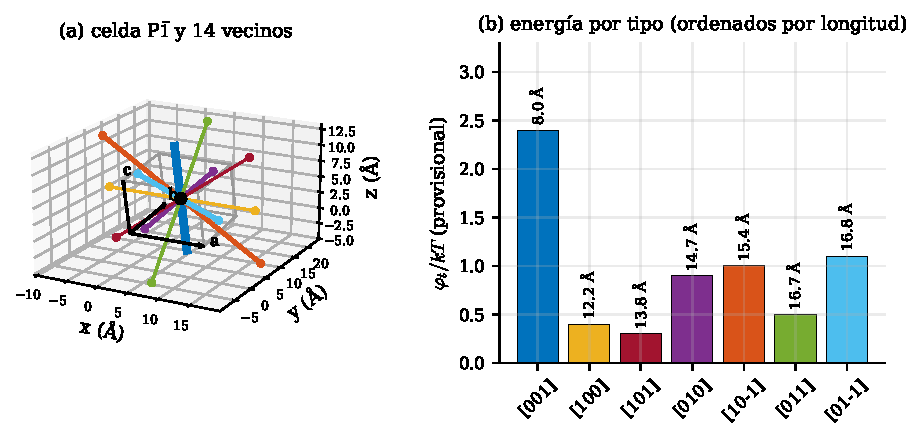
\includegraphics[width=\linewidth]{celda_bh_enlaces.pdf}
\caption{(a) Celda P$\overline1$ de \bh{} (aristas grises, vectores $\vect a,\vect b,\vect c$) y los
14 vecinos $\vect r\pm\vect v_t$ de una unidad (punto negro); el grosor de cada segmento es
proporcional a $\varphi_t$ y los colores son los de (b). (b) Energía efectiva \emph{provisional}
$\varphi_t/kT$ de cada tipo, ordenados por longitud del vector de enlace. Generado por
\code{make\_figures.py} con \code{presets.beta\_hematin()}.}
\label{fig:celdabh}
\end{figure}

% =============================================================================
\section{Grafo cristalino y energía de un sitio}
\label{sec:grafo}
% =============================================================================

\subsection{Tipos de enlace y energía}

Un \code{BondType} es un vector de red $\vect v_t\in\mathbb Z^3$, $\vect v_t\neq\vect 0$, con energía
$\varphi_t>0$ (en $kT$, atractiva). Une la unidad en $\vect r$ con \emph{dos} vecinas,
$\vect r+\vect v_t$ y $\vect r-\vect v_t$; por eso $\vect v$ y $-\vect v$ son el mismo tipo y el
constructor de \code{CrystalGraph} rechaza duplicados. Con $T$ tipos, la coordinación es $z=2T$ (6 en
Kossel, 14 en \bh{}), y el \emph{alcance} $\max_t\|\vect v_t\|_\infty$ fija el ancho mínimo del borde
de la caja (\S\ref{sec:caja}). Si $n_t(\vect r)\in\{0,1,2\}$ es el número de vecinos ocupados del
tipo $t$, la energía de enlace de un sitio y la energía de una configuración $\{o_{\vect r}\}$ son
\begin{equation}
E(\vect r)=\sum_{t=0}^{T-1} n_t(\vect r)\,\varphi_t,\qquad
U=-\sum_{\text{pares }(\vect r,\vect r\pm\vect v_t)}\varphi_t\,o_{\vect r}\,o_{\vect r\pm\vect v_t}.
\label{eq:E}
\end{equation}

\begin{supuesto}{S2. Energía aditiva por pares, de corto alcance y efectiva en solución}
La energía es una suma de pares por tipo de enlace, sin términos de muchos cuerpos, sin relajación
de la red ni deformación elástica, y sin dependencia del entorno químico. Las $\varphi_t$ son
energías libres \emph{efectivas} en solución (incluyen solvatación), en unidades de $kT$, y la
temperatura solo entra a través de ellas: multiplicar todas por un factor (\code{scale}) equivale
a cambiar la temperatura efectiva.
\end{supuesto}

\subsection{Código de vecindad}

Toda la información que determina la tasa de un sitio está en el vector $(n_0,\dots,n_{T-1})$, que
se codifica en un entero en base 3 (\code{encode}/\code{decode}):
\begin{equation}
c(\vect r)=\sum_{t=0}^{T-1} n_t(\vect r)\,3^t,\qquad 0\le c\le c_{\mathrm{full}}=\sum_t 2\cdot 3^t=3^T-1 .
\label{eq:codigo}
\end{equation}
Hay $3^T$ códigos (27 en Kossel, 2187 en \bh{}). El código distingue la \emph{orientación} (el tipo
de enlace) pero no cuál de $\vect r\pm\vect v_t$ está ocupado, información que no afecta a la
energía. Como el motor guarda los códigos en \code{int32}, $T\le19$ ($3^{19}<2^{31}<3^{20}$).
La regla de actualización es local: si se ocupa $\vect r$, cada vecino $\vect r\pm\vect v_t$ gana un
vecino del tipo $t$ y su código aumenta en $3^t$ (Fig.~\ref{fig:codigo}).

\begin{figure}[t]
\centering
\begin{tikzpicture}[scale=0.82,
  occ/.style={circle,fill=black,inner sep=2.1pt},
  emp/.style={circle,draw=black,fill=white,inner sep=2.1pt}]
  \foreach \p/\q in {0/0,8.6/0}{
    \begin{scope}[xshift=\p cm]
      \foreach \i in {-2,...,2}{\foreach \j in {-2,...,2}{\fill[black!25] (\i,\j) circle (1.3pt);}}
    \end{scope}}
  % (a) sitio vacío y su código
  \draw[azul,very thick] (0,0) -- (1,0);  \draw[azul,very thick] (0,0) -- (-1,0);
  \draw[naranja,very thick] (0,0) -- (0,-1); \draw[naranja,thick,dotted] (0,0) -- (0,1);
  \draw[verde!80!black,very thick] (0,0) -- (-1,-1); \draw[verde!80!black,thick,dotted] (0,0) -- (1,1);
  \node[occ] at (1,0) {}; \node[occ] at (-1,0) {}; \node[occ] at (0,-1) {}; \node[occ] at (-1,-1) {};
  \node[emp] at (0,1) {}; \node[emp] at (1,1) {};
  \node[draw=carmin,thick,fill=white,minimum size=7pt,inner sep=0pt] at (0,0) {};
  \node[font=\scriptsize,azul] at (1.55,-0.3) {$t=0$: $[10]$};
  \node[font=\scriptsize,naranja] at (0.55,-1.45) {$t=1$: $[01]$};
  \node[font=\scriptsize,verde!60!black] at (1.75,1.3) {$t=2$: $[11]$};
  \node[font=\small,align=center] at (0,-3.1) {(a) $\vect n=(2,1,1)$\\$c=2\cdot3^0+1\cdot3^1+1\cdot3^2=14$\\$E=2\varphi_0+\varphi_1+\varphi_2$};
  % (b) actualización incremental tras la unión
  \begin{scope}[xshift=8.6cm]
    \foreach \i/\j/\w/\col in {1/0/1/azul,-1/0/1/azul,0/1/3/naranja,0/-1/3/naranja,1/1/9/verde!70!black,-1/-1/9/verde!70!black}{
      \draw[-{Stealth},thick,\col] (0,0) -- ({0.82*\i},{0.82*\j});
      \node[font=\scriptsize,\col,fill=white,inner sep=0.5pt] at ({1.32*\i+0.12},{1.32*\j+0.12}) {$+\w$};}
    \node[occ,fill=carmin] at (0,0) {};
    \node[font=\small,align=center] at (0,-3.1) {(b) al unirse en $\vect r$:\\$c(\vect r\pm\vect v_t)\mathrel{+}=3^t$;\\se reclasifican $2T+1=7$ sitios};
  \end{scope}
\end{tikzpicture}
\caption{Código de vecindad en un ejemplo 2D con $T=3$ tipos ($[10]$, $[01]$, $[11]$, pesos $1,3,9$).
Línea continua: vecino ocupado; punteada: vacío. (a) Sitio vacío candidato a unión. (b) Tras la
unión, los $2T$ vecinos cambian su código en $\pm3^t$ y nada más cambia: es la base del algoritmo
incremental (\S\ref{sec:incremental}).}
\label{fig:codigo}
\end{figure}

\subsection{Energía de red y posición de media-cristal (kink)}
\label{sec:kink}

Una unidad del interior tiene $n_t=2$ para todo $t$ y energía $2\sum_t\varphi_t$; como cada enlace se
comparte entre dos unidades, la energía de red por unidad es $\Ecr=\sum_t\varphi_t$. La
\emph{posición de media-cristal} (kink) de Kossel y Stranski~\cite{kossel1927,stranski1928} es aquella
en la que la unidad tiene ocupado exactamente medio cristal: si se ordenan los sitios con cualquier
orden total compatible con las traslaciones (p.\,ej.\ lexicográfico en $(i,j,k)$), para cada
$\vect v_t\neq0$ exactamente uno de $\vect r\pm\vect v_t$ precede a $\vect r$. Así $n_t=1$ para todo
$t$ y
\begin{equation}
\Ekink=\sum_t\varphi_t=\Ecr .
\label{eq:kink}
\end{equation}
Unirse a un kink reproduce el kink (paso repetible): es la referencia termodinámica del cristal. La
Fig.~\ref{fig:kossel} muestra los sitios típicos de una superficie de Kossel.

\begin{figure}[t]
\centering
\begin{tikzpicture}[x={(0.78cm,0cm)},y={(0.38cm,0.27cm)},z={(0cm,0.78cm)}]
  \foreach \y in {4,3}{
    \foreach \x in {0,...,6}{\cubo{\x}{\y}{0}{azul}}
    \foreach \x in {0,...,6}{\cubo{\x}{\y}{1}{azul}}}
  \foreach \x in {0,...,6}{\cubo{\x}{2}{0}{azul}}
  \foreach \x in {0,...,2}{\cubo{\x}{2}{1}{azul}}
  \foreach \x in {0,...,6}{\cubo{\x}{1}{0}{azul}}
  \foreach \x in {0,...,6}{\cubo{\x}{0}{0}{azul}}
  \cubo{5}{0}{1}{naranja}
  \tikzset{sitio/.style={circle,draw=carmin,fill=carmin!45,inner sep=1.8pt}}
  \node[sitio] (K) at (3.5,2.5,1.4) {};
  \node[sitio] (S) at (5.5,2.5,1.4) {};
  \node[sitio] (T) at (1.5,0.5,1.25) {};
  \node[font=\scriptsize,anchor=east] (Kl) at (-0.6,3.0,3.2) {kink: $n=3$, $E=\Ekink$};
  \node[font=\scriptsize,anchor=west] (Sl) at (7.6,3.0,3.2) {borde de escalón: $n=2$};
  \node[font=\scriptsize,anchor=east] (Tl) at (-0.8,0.0,0.6) {sobre la terraza: $n=1$};
  \node[font=\scriptsize,anchor=west] (Al) at (8.0,0.0,0.9) {adátomo: $n=1$, despegue rápido};
  \draw[carmin] (Kl.east) -- (K);
  \draw[carmin] (Sl.west) -- (S);
  \draw[carmin] (Tl.east) -- (T);
  \draw[naranja] (Al.west) -- (6.0,0.5,1.5);
\end{tikzpicture}
\caption{Superficie de Kossel (cara $\{100\}$) con terraza, escalón y kink. Los círculos marcan sitios
vacíos de unión y su número de vecinos ocupados $n$; el cubo naranja es un adátomo. Con $\varphi$
igual en las tres direcciones, $E=n\varphi$ y $\Ekink=3\varphi$.}
\label{fig:kossel}
\end{figure}

\subsection{Teoría de Hartman--Perdok: energía de capa, de unión y carácter de cara}
\label{sec:hp}

Con una unidad por celda y $(hkl)$ coprimos, la capa de espesor $d_{hkl}$ contiene un solo plano
reticular. Un enlace de tipo $t$ con $p_t=\vect h\cdot\vect v_t$ une el plano $m$ con $m\pm p_t$:
\begin{equation}
\Eslice(hkl)=\sum_{t:\,p_t=0}\varphi_t,\qquad
\Eatt(hkl)=\sum_{t:\,p_t\neq0}\varphi_t,\qquad \Eslice+\Eatt=\Ecr .
\label{eq:hp}
\end{equation}
Justificación: si el cristal ocupa todos los planos $\le m-1$ y se completa el plano $m$, cada unidad
nueva tiene, para cada $t$ con $p_t\neq0$, exactamente uno de sus dos vecinos de tipo $t$ en un plano
inferior (ocupado) y el otro en uno superior (vacío): libera $\varphi_t$ al unirse. Los enlaces con
$p_t=0$ quedan dentro de la capa y contribuyen $2\varphi_t/2=\varphi_t$ por unidad. \code{face\_table}
reporta $\Eatt$ con signo negativo, como en la literatura. El \emph{modelo de energía de unión} de
Hartman y Bennema~\cite{hartman1980} supone
\begin{equation}
R_{hkl}\propto|\Eatt(hkl)|,
\label{eq:ratt}
\end{equation}
que da la ``forma de energía de unión'' (\code{attachment\_energy\_morphology}).

\paragraph{Carácter F/S/K.} Una cara es plana (F) si la capa contiene una red 2D conexa de cadenas
periódicas de enlaces (PBC)~\cite{hartman1955}. Con una unidad por celda cada tipo de enlace genera
por sí solo una cadena recta infinita $\vect r+\mathbb Z\vect v_t$, así que basta el rango de los
vectores de la capa con $\varphi_t>0$: rango 2, cara \textbf{F}; rango 1, \textbf{S} (escalonada);
ninguno, \textbf{K} (con kinks) (\code{face\_character}). En Kossel, $\{100\}$ es F, $\{110\}$ S y
$\{111\}$ K, con $|\Eatt|=\varphi,2\varphi,3\varphi$ (Fig.~\ref{fig:hp}); con enlaces diagonales
$[110]$, $[1\bar10]$, la $\{110\}$ pasa a F (\code{test\_second\_neighbours\_make\_110\_flat}). Con base
$>1$ (F6) el rango deja de bastar y hace falta el criterio de redes conexas~\cite{grimbergen1998}.

\begin{figure}[t]
\centering
\begin{tikzpicture}[scale=0.58]
  % (a) cara (10)
  \fill[azul!12] (-0.5,-2.45) rectangle (0.5,2.45);
  \foreach \j in {-2,...,2}{\draw[thick,azul,dashed] (-1,\j) -- (1,\j);}
  \foreach \j in {-2,...,1}{\draw[very thick,naranja] (0,\j) -- (0,{\j+1});}
  \foreach \i in {-2,...,2}{\foreach \j in {-2,...,2}{\fill (\i,\j) circle (2.2pt);}}
  \draw[-{Stealth},carmin,thick] (0.6,2.75) -- (1.7,2.75) node[right,font=\small] {$\hat{\vect n}_{10}$};
  \node[font=\small,align=center] at (0,-3.6) {(a) cara $(10)$:\\$\Eslice=\varphi_{[01]}$, $\Eatt=\varphi_{[10]}$};
  % (b) cara (11)
  \begin{scope}[xshift=8.4cm]
    \fill[azul!12] (-2.45,1.95) -- (-1.95,2.45) -- (2.45,-1.95) -- (1.95,-2.45) -- cycle;
    \begin{scope}
      \clip (-2.45,-2.45) rectangle (2.45,2.45);
      \foreach \i in {-2,...,2}{
        \draw[thick,azul,dashed] ({\i-1},{-\i}) -- ({\i+1},{-\i});
        \draw[thick,naranja,dashed] (\i,{-\i-1}) -- (\i,{-\i+1});}
    \end{scope}
    \foreach \i in {-2,...,2}{\foreach \j in {-2,...,2}{\fill (\i,\j) circle (2.2pt);}}
    \draw[-{Stealth},carmin,thick] (1.4,1.4) -- (2.2,2.2) node[above right,font=\small] {$\hat{\vect n}_{11}$};
    \node[font=\small,align=center] at (0,-3.6) {(b) cara $(11)$: $\Eslice=0$,\\$\Eatt=\varphi_{[10]}+\varphi_{[01]}$};
  \end{scope}
  \node[font=\small,align=left,anchor=north west] at (12.2,2.4) {color: tipo de enlace\\ \textcolor{azul}{$[10]$}, \textcolor{naranja}{$[01]$}\\[2pt]\rule[2pt]{14pt}{1.2pt}\ dentro de la capa\\- - -\ \ cruza la capa\\[8pt]Kossel 3D ($\varphi$ igual):\\$\{100\}$ F, $|\Eatt|=\varphi$\\$\{110\}$ S, $|\Eatt|=2\varphi$\\$\{111\}$ K, $|\Eatt|=3\varphi$};
\end{tikzpicture}
\caption{Capas de Hartman--Perdok en una red cuadrada (corte 2D). La banda sombreada es la capa de
espesor $d_{hkl}$ que contiene un plano. Los enlaces que la cruzan son los que se liberan al unirse
una capa nueva ($\Eatt$); los que quedan dentro, $\Eslice$. En 3D el criterio F es rango 2.}
\label{fig:hp}
\end{figure}

\paragraph{Energías provisionales de \bh{}.} \code{BETA\_HEMATIN\_ENERGIES\_PROVISIONAL} asigna una
energía a cada uno de los siete vectores más cortos (Tabla~\ref{tab:bh}). \textbf{No salen de ningún
cálculo}: se eligieron solo para que $|\Eatt|$ ordene las caras como se observa,
$(100)<(010)<(011)<(001)<(01\bar1)$, con todas las caras observadas de tipo F
(\code{test\_beta\_hematin\_provisional\_ordering}). $\Ecr=6.6\,kT$.

\begin{table}[t]
\centering\small
\caption{\bh{}: enlaces (izquierda) y teoría de energía de unión (derecha), con las energías
provisionales. $R_{\rm att}$ relativa a la cara más lenta, según~\eqref{eq:ratt}.}
\label{tab:bh}
\begin{tabular}{@{}lccl@{}}
\toprule
Enlace & $|\vect v_t|$ (Å) & $\varphi_t/kT$ & Interpretación\\
\midrule
$[001]$ & 8.04 & 2.4 & traslación más corta; eje de aguja\\
$[10\bar1]$ & 15.38 & 1.0 & cadenas de puentes de H\\
$[01\bar1]$ & 16.77 & 1.1 & \\
$[010]$ & 14.68 & 0.9 & \\
$[011]$ & 16.71 & 0.5 & \\
$[100]$ & 12.20 & 0.4 & \\
$[101]$ & 13.79 & 0.3 & \\
\bottomrule
\end{tabular}\hfill
\begin{tabular}{@{}lccccc@{}}
\toprule
Cara & $d_{hkl}$ (Å) & $\Eslice$ & $\Eatt$ & $R_{\rm att}$ & Car.\\
\midrule
$(100)$ & 11.99 & 4.9 & $-1.7$ & 1.00 & F\\
$(010)$ & 14.54 & 4.1 & $-2.5$ & 1.47 & F\\
$(110)$, $(1\bar10)$ & 8.68, 9.96 & 2.4 & $-4.2$ & 2.47 & S\\
$(101)$ & 6.30 & 1.9 & $-4.7$ & 2.76 & F\\
$(011)$ & 6.94 & 1.5 & $-5.1$ & 3.00 & F\\
$(001)$ & 7.98 & 1.3 & $-5.3$ & 3.12 & F\\
$(10\bar1)$ & 7.05 & 1.2 & $-5.4$ & 3.18 & F\\
$(01\bar1)$ & 7.06 & 0.9 & $-5.7$ & 3.35 & F\\
\bottomrule
\end{tabular}
\end{table}

% =============================================================================
\section{Termodinámica y modelos de tasas}
\label{sec:tasas}
% =============================================================================

\subsection{Fuerza impulsora y energía libre de unión}

La fuerza impulsora es $\dmu=\mu_{\rm sol}-\mu_{\rm cr}$ en unidades de $kT$ ($>0$ crece). Con la
convención de la línea estática del proyecto (\code{delta\_mu\_from\_sigma}, exige $\sigma>-1$):
\begin{equation}
\dmu=S=\ln\frac{C}{C_{\rm eq}}=\ln(1+\sigma),\qquad \sigma=\frac{C}{C_{\rm eq}}-1 .
\label{eq:dmu}
\end{equation}
Pasar una unidad de la solución a un sitio de energía de enlace $E$ cambia la energía libre en
\begin{equation}
\Delta G(E)=-\bigl[\dmu+(E-\Ekink)\bigr],
\label{eq:dG}
\end{equation}
de modo que a $\dmu=0$ el kink no gana ni pierde; un sitio con $E>\Ekink$ (p.\,ej.\ un hueco en una
terraza) es favorable incluso en subsaturación, y uno con $E<\Ekink$ (un adátomo) desfavorable salvo
que $\dmu>\Ekink-E$.

\begin{supuesto}{S3. Solución ideal, reservorio infinito y control por superficie}
$\dmu$ es constante en el tiempo (sin agotamiento, D5; la API \code{set\_delta\_mu} existe para F4) y
uniforme sobre todo el cristal (sin gradientes de concentración en la solución): el crecimiento está
limitado por la cinética de superficie, no por el transporte. La solución no se simula: es un
reservorio implícito.
\end{supuesto}
\begin{supuesto}{S4. El kink como referencia: $\mu_{\rm cr}=-\Ecr$}
La energía libre de la unidad en el cristal es la de la posición kink; se desprecian contribuciones
vibracionales y de entropía de la unidad en la red (o se absorben en $\varphi_t$ y $k_0$).
\end{supuesto}

\subsection{Balance detallado y equivalencia con un gas de red}
\label{sec:gasred}

Toda tasa con balance detallado debe cumplir
\begin{equation}
\frac{k^+(E)}{k^-(E)}=e^{-\Delta G(E)}=e^{\dmu+E-\Ekink}.
\label{eq:db}
\end{equation}
Si se une una unidad, la suma de enlaces de~\eqref{eq:E} aumenta en $E$ y $N$ en 1, así que~\eqref{eq:db}
equivale a que, en cada transición permitida en los dos sentidos, el cociente de probabilidades sea el de
\begin{equation}
P(\{o\})\propto e^{-\mathcal H},\qquad
\mathcal H=-\!\!\sum_{\text{pares}}\varphi_t\,o_{\vect r}o_{\vect r'}-\mu_{\rm LG}N,\qquad
\mu_{\rm LG}=\dmu-\Ekink ,
\label{eq:lg}
\end{equation}
un \textbf{gas de red gran canónico}. Las únicas transiciones sin inversa son las de unidades sueltas y,
con \code{allow\_enclosed=True}, las de huecos cerrados (observación técnica 1 de \S\ref{sec:supuestos}). Con $o=(1+s)/2$ se obtiene un Ising con acoplamientos
$J_t=\varphi_t/4$ y campo proporcional a $\mu_{\rm LG}+\sum_t\varphi_t=\dmu$: la coexistencia
cristal--solución (campo nulo, punto de simetría partícula--hueco $\mu_{\rm LG}=-\sum_t\varphi_t$)
cae exactamente en $\dmu=0$. Es una comprobación de consistencia de~\eqref{eq:dG} y permite usar
resultados conocidos de Ising 3D para Kossel ($J=\varphi/4$): el gas de red solo distingue cristal y
solución por debajo del punto crítico, $\varphi/kT>4K_c\approx0.89$, y la cara $\{100\}$ es rugosa en
equilibrio para $\varphi/kT\lesssim4K_R\approx1.6$ ($K_R\approx0.41$~\cite{hasenbusch1996}; el modelo
SOS da prácticamente lo mismo, $kT_R/\varphi\approx0.62$~\cite{weeks1979}).\footnote{Valores de la
literatura, no calculados en este proyecto. El notebook~01 (\S3.2) escribe ``$\varphi/kT\approx1.2$
($J=\varphi/2$, $K_R\approx0.62$)'', que toma $0.62$ como $J/kT$; ese número es en realidad $kT_R/\varphi$.
La conclusión cualitativa del notebook no cambia: $\varphi=1$ queda en el lado rugoso y $\varphi=2,3$ en
el liso con cualquiera de los dos valores.}

\subsection{Familia \texorpdfstring{\code{SplitRates}}{SplitRates}}

Con $x=E-\Ekink$ y dos parámetros $a,b\in[0,1]$ que reparten la fuerza impulsora y el cambio de
energía entre unión y despegue:
\begin{equation}
k^+(E)=k_0\,e^{\,a\dmu+b\,x},\qquad k^-(E)=k_0\,e^{-(1-a)\dmu-(1-b)\,x}
\quad\Longrightarrow\quad \frac{k^+}{k^-}=e^{\dmu+x}=e^{-\Delta G},
\label{eq:split}
\end{equation}
que cumple~\eqref{eq:db} para cualquier $(a,b)$: todos los miembros de la familia tienen el
\emph{mismo equilibrio} y distinta cinética (Fig.~\ref{fig:tasas}). Casos con nombre:
\begin{itemize}
\item \textbf{Gilmer} ($a=1,b=0$, \code{SplitRates.gilmer}): $k^+=k_0e^{\dmu}$ igual en todos los
sitios y $k^-=k_0e^{\Ekink-E}$; en Kossel, $k^-_n=k_0e^{(3-n)\varphi}$. Es el modelo clásico de
Gilmer y Bennema~\cite{gilmer1972}.
\item \textbf{Simétrico} ($a=b=\tfrac12$, \code{SplitRates.symmetric}): $k^\pm=k_0e^{\pm(\dmu+x)/2}$.
Es el tipo de reparto de MONTY y CrystalGrower; la forma exacta de sus ecuaciones \emph{no} se ha
verificado (D2).
\item \textbf{Intermedio} ($b>0$): la unión se vuelve selectiva por sitio (como la tasa adaptativa de
Nagpal et al.~\cite{nagpal2024}) sin romper el balance detallado.
\end{itemize}
En lenguaje de estado de transición (Fig.~\ref{fig:barrera}), $a$ y $b$ fijan qué fracción de la
caída de energía libre se traslada a la barrera de unión.

\begin{figure}[t]
\centering
\begin{tikzpicture}[x=0.95cm,y=0.95cm]
  \draw[-{Stealth}] (0,-1.9) -- (0,2.3) node[above,font=\small] {$G/kT$};
  \draw[-{Stealth}] (0,-1.9) -- (8.3,-1.9) node[below left,font=\small] {coordenada de reacción};
  \draw[very thick,navy] (0.3,0) -- (1.2,0) .. controls (2.2,0) and (2.6,1.6) .. (3.4,1.6)
        .. controls (4.2,1.6) and (4.7,-1.3) .. (5.7,-1.3) -- (6.6,-1.3);
  \draw[dashed,gris] (1.2,0) -- (7.8,0);
  \draw[dashed,gris] (2.4,1.6) -- (7.8,1.6);
  \draw[{Stealth}-{Stealth},azul,thick] (1.8,0) -- (1.8,1.6) node[midway,left,font=\scriptsize,align=right] {$\ln\frac{k_0}{k^+}=$\\$-a\dmu-b\,x$};
  \draw[{Stealth}-{Stealth},naranja,thick] (5.4,-1.3) -- (5.4,1.6) node[pos=0.62,right,font=\scriptsize,align=left] {$\ln\frac{k_0}{k^-}=$\\$(1-a)\dmu+(1-b)x$};
  \draw[{Stealth}-{Stealth},carmin,thick] (7.6,0) -- (7.6,-1.3) node[midway,right,font=\scriptsize] {$\Delta G=-(\dmu+x)$};
  \node[font=\scriptsize,align=center,below] at (0.75,-0.08) {solución +\\sitio vacío};
  \node[font=\scriptsize,align=center,above] at (6.35,-1.25) {unidad unida\\(energía $E$)};
  \node[font=\scriptsize,align=center,above] at (3.4,1.65) {estado de transición};
\end{tikzpicture}
\caption{Lectura de~\eqref{eq:split} como teoría de estado de transición (esquema; $x=E-\Ekink$). La
referencia de la barrera es la que define $k_0$, así que una ``barrera'' puede ser negativa. La
diferencia entre las dos barreras es siempre $-\Delta G$: el balance detallado no depende de $(a,b)$.}
\label{fig:barrera}
\end{figure}

\begin{figure}[t]
\centering
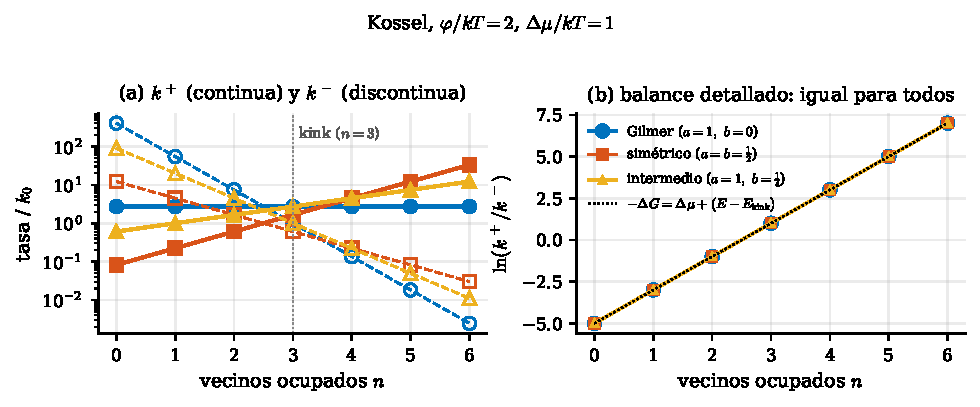
\includegraphics[width=\linewidth]{tasas_vs_enlaces.pdf}
\caption{(a) $k^+$ y $k^-$ de tres miembros de \code{SplitRates} frente al número de vecinos
ocupados en Kossel ($E=n\varphi$, $\Ekink=3\varphi$). Gilmer: unión plana, todo el contraste en el
despegue; simétrico: la unión favorece a los sitios muy coordinados. (b) $\ln(k^+/k^-)$ es idéntico
para todos (balance detallado~\eqref{eq:db}). Calculado con \code{kmc3d.rates}.}
\label{fig:tasas}
\end{figure}

\begin{supuesto}{S5. Tasas de tipo Arrhenius con un único prefactor}
Un único $k_0$ para todos los sitios y eventos (el tiempo se mide en $1/k_0$, D7), dependencia del
sitio solo a través de $E$ (es decir, del código), y reparto $(a,b)$ constante (D2). Sin barreras de
desolvatación dependientes de la cara ni efectos estéricos de orientación.
\end{supuesto}

\subsection{\texorpdfstring{\code{AdaptiveRates}}{AdaptiveRates} y comparación con la línea 2D}
\label{sec:adaptive}

Para comparar con el motor estático 2D (forma de Nagpal~\cite{nagpal2024}) se implementa
\begin{equation}
k^+=K_0\exp\Bigl(S+\frac{1}{S}\sum_t n_t\delta_t\Bigr),\qquad k^-=K_0\,e^{\varphi_0-E},\qquad S=\dmu,
\label{eq:adaptive}
\end{equation}
con $\varphi_0=\Ekink$ por defecto y $\delta_t$ por tipo de enlace. Si $|S|<10^{-12}$ se usa
$S_{\rm eff}=\pm10^{-12}$: la forma adaptativa diverge cuando $S\to0$, propiedad del modelo original.
\textbf{No cumple balance detallado}: $\ln(k^+/k^-)=S+\sum_tn_t\delta_t/S-\varphi_0+E$ no es de la
forma~\eqref{eq:db} salvo $\delta_t=0$, $\varphi_0=\Ekink$. Sirve solo para comparar.

En la cara (001) de un cristal cúbico con $\delta_z=0$ y $\varphi_0=\varphi_{2D}+\varphi_z$,
\eqref{eq:adaptive} coincide con $r_a$, $r_d$ de \code{KMC\_BKL\_Static} \emph{donde coinciden las
convenciones de conteo} (Fig.~\ref{fig:conteo}). El 2D cuenta un vecino lateral solo si su altura es
\emph{exactamente} el nivel del sitio; el 3D cuenta el contacto geométrico. Para la unión sobre una
columna de altura $h$ coinciden si ningún vecino supera $h+1$; para el despegue, si ninguno supera $h$
(\code{TestAdaptiveVsStatic2D}, que además comprueba que la diferencia existe). La física del 2D no se
ha tocado (regla del proyecto): la diferencia queda como decisión D6.

\begin{figure}[t]
\centering
\begin{tikzpicture}[x=0.45cm,y=0.45cm,u/.style={draw=black!70,fill=azul!35,line width=0.3pt}]
  \foreach \x/\h in {0/3,1/4,2/3,3/6,4/4}{\foreach \z in {1,...,\h}{\draw[u] (\x,{\z-1}) rectangle ++(1,1);}}
  \draw[thick] (-0.4,0) -- (5.4,0);
  \draw[carmin,thick,dashed,fill=carmin!10] (2,3) rectangle ++(1,1);
  \fill[carmin] (2.5,3.5) circle (2.5pt);
  \draw[verde!70!black,very thick] (2.5,3.5) -- (1.5,3.5);
  \draw[naranja,very thick] (2.5,3.5) -- (3.5,3.5);
  \draw[gris,very thick] (2.5,3.5) -- (2.5,2.5);
  \node[font=\scriptsize,anchor=west,align=left] at (6.2,5.2) {sitio de unión sobre la columna central ($h=3$, nivel 3)};
  \node[font=\scriptsize,anchor=west,align=left,verde!50!black] at (6.2,4.1) {izquierda: altura $4=h+1$ $\Rightarrow$ cuenta en 2D y en 3D};
  \node[font=\scriptsize,anchor=west,align=left,naranja] at (6.2,3.0) {derecha: altura $6>h+1$ $\Rightarrow$ cuenta en 3D (contacto), no en 2D (\code{==})};
  \node[font=\scriptsize,anchor=west,align=left,gris] at (6.2,1.9) {abajo: enlace vertical $\varphi_z$, en los dos};
  \node[font=\scriptsize,anchor=west,align=left] at (6.2,0.8) {3D: 2 enlaces laterales; 2D: 1 $\Rightarrow$ tasas distintas (D6)};
\end{tikzpicture}
\caption{Diferencia de convención de conteo entre la línea (2+1)D y la 3D, en un corte de una
superficie SOS. Las tasas coinciden exactamente en los sitios donde ningún vecino es más alto que
$h+1$ (unión) o $h$ (despegue).}
\label{fig:conteo}
\end{figure}

\paragraph{Implementación.} Las tasas dependen solo del código, así que \code{RateModel} las guarda
en caché por código (y las energías por código): el motor solo las pide al crear una clase nueva.
\code{set\_delta\_mu} vacía la caché de tasas (no la de energías). Todas las exponenciales pasan por
\code{src.common.numerics.\_safe\_exp}, que recorta el argumento a $|x|\le700$ para evitar
desbordamientos. \code{rates\_from\_dict} reconstruye el modelo desde la metadata (\code{split},
\code{gilmer}, \code{symmetric}, \code{adaptive}).

% =============================================================================
\section{Algoritmo kMC: BKL (\emph{n-fold way}) incremental}
\label{sec:bkl}
% =============================================================================

\subsection{Ecuación maestra y kMC sin rechazo}

La evolución es un proceso de Markov de saltos con ecuación maestra
\begin{equation}
\frac{dP(\sigma,t)}{dt}=\sum_{\sigma'}\bigl[W(\sigma'\!\to\sigma)P(\sigma',t)-W(\sigma\to\sigma')P(\sigma,t)\bigr].
\label{eq:master}
\end{equation}
El algoritmo BKL~\cite{bortz1975} la integra exactamente (sin rechazo ni discretización del tiempo).
Desde un estado con eventos de tasas $r_i$ y tasa total $W=\sum_ir_i$, el tiempo hasta el siguiente
evento es exponencial, $P(\Delta t>\tau)=e^{-W\tau}$, y el evento $i$ ocurre con probabilidad $r_i/W$:
\begin{equation}
\Delta t=-\frac{\ln(1-u_1)}{W}\cdot\code{time\_scale},\qquad
P(\text{evento }i)=\frac{r_i}{W},\qquad u_1\in[0,1).
\label{eq:dt}
\end{equation}
Se usa $1-u_1\in(0,1]$ para evitar $\ln0$; la distribución es la misma.

\begin{supuesto}{S6. Eventos elementales: solo unión y despegue de una unidad}
Proceso markoviano (sin memoria) con dos tipos de evento. No hay difusión superficial (F4), ni
unión o desprendimiento de agregados, ni nucleación homogénea en la solución, ni etapas químicas
o conformacionales (el dímero de \bh{} llega ya formado). Un fragmento desconectado del cristal
no se mueve como cuerpo rígido: solo pierde o gana unidades una a una.
\end{supuesto}

\subsection{Eventos elegibles}

La Tabla~\ref{tab:eventos} define qué evento admite cada sitio según su ocupación y su código.

\begin{table}[h]
\centering\small
\caption{Eventos elegibles por sitio (\code{reclass} y \code{\_install}).}
\label{tab:eventos}
\begin{tabularx}{\linewidth}{@{}llY@{}}
\toprule
Sitio & Código & Evento\\
\midrule
vacío & $c=0$ & ninguno: la solución no ``llega'' a sitios sin vecinos (S7)\\
vacío & $0<c<c_{\rm full}$ & unión, con tasa $k^+(c)$\\
vacío & $c=c_{\rm full}$ & ninguno por defecto (hueco cerrado, \code{allow\_enclosed=False}, D4); unión si \code{True}\\
ocupado & $c<c_{\rm full}$ (incluido $c=0$) & despegue, con tasa $k^-(c)$; una unidad suelta también se despega (D8)\\
ocupado & $c=c_{\rm full}$ & ninguno: unidad del interior, sin contacto con la solución\\
\bottomrule
\end{tabularx}
\end{table}

\begin{supuesto}{S7. Llegada local y accesibilidad por sitio}
Una unidad solo se une a un sitio con al menos un vecino ocupado, y cualquier sitio así es accesible
desde la solución. La accesibilidad se comprueba \emph{sitio a sitio}: solo se excluye el hueco con
\emph{todos} sus $2T$ vecinos ocupados. Una cavidad de varios sitios sellada (Fig.~\ref{fig:sos3d}b)
sí recibe unidades. Una unidad del interior ($c=c_{\rm full}$) nunca se despega: no se crean vacantes
en el volumen.
\end{supuesto}

\subsection{Clases de eventos}

Como la tasa de un sitio depende solo de su código y del tipo de evento $\tau$ (0 unión, 1 despegue),
todos los sitios con la misma clave
\begin{equation}
\kappa=2c+\tau
\label{eq:clave}
\end{equation}
tienen la misma tasa $r_\kappa$. Con $n_\kappa$ miembros, $W=\sum_\kappa n_\kappa r_\kappa$, y elegir
primero la clase con probabilidad $n_\kappa r_\kappa/W$ y después un miembro uniforme da a cada sitio
la probabilidad $r_\kappa/W$ de~\eqref{eq:dt}: es exacto. Hay como mucho $2\cdot3^T$ claves (54 en
Kossel, 4374 en \bh{}), pero las clases se crean solo cuando aparece un sitio con esa clave
(Fig.~\ref{fig:clases}). Cada clase guarda sus miembros en una lista; los arrays \code{cls\_of[s]} y
\code{pos\_of[s]} dan la clase y la posición de cada sitio, de modo que insertar y quitar cuestan
$O(1)$ (borrado \emph{swap-and-pop}, Fig.~\ref{fig:fenwick}a).

\begin{figure}[t]
\centering
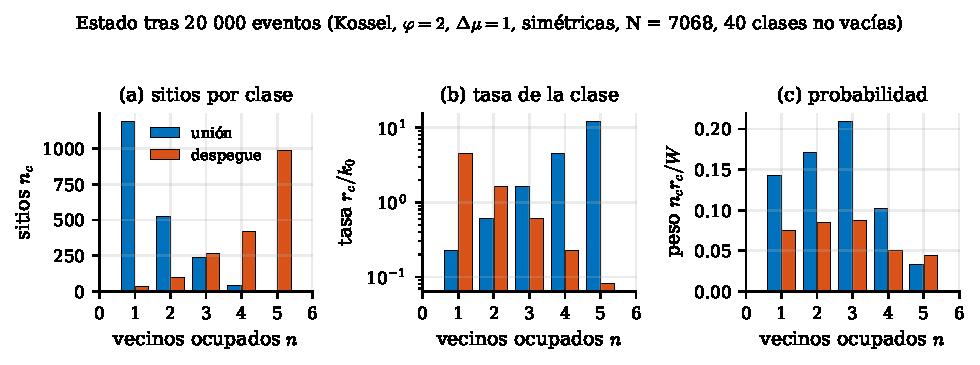
\includegraphics[width=\linewidth]{clases_estado.pdf}
\caption{Clases \emph{n-fold way} de un estado real (Kossel, $\varphi=2$, $\dmu=1$, simétricas, tras
20\,000 eventos desde un cubo de lado 10), agrupadas por número de vecinos. Los sitios abundantes
(uniones con $n=1$) no dominan necesariamente: el peso $n_\kappa r_\kappa$ es el que decide.}
\label{fig:clases}
\end{figure}

\subsection{Árbol de Fenwick}

El peso $w_\kappa=n_\kappa r_\kappa$ de cada clase se guarda en un árbol de Fenwick~\cite{fenwick1994}
(\code{fenwick.py}). Con índices desde 1 y $\ell(i)=i\,\&\,(-i)$ (el bit menos significativo),
\begin{equation}
T_i=\sum_{j=i-\ell(i)+1}^{i}w_j,\qquad
\textstyle\sum_{j\le i}w_j=T_i+T_{i-\ell(i)}+\cdots,\qquad
\text{\code{add}}(i,\delta):\ T_i\mathrel{+}=\delta,\ i\leftarrow i+\ell(i).
\label{eq:fenwick}
\end{equation}
\code{find}$(u W)$ desciende desde la mayor potencia de 2 $\le K$ y devuelve la menor clase con suma
acumulada $>uW$ (Fig.~\ref{fig:fenwick}b). Las tres operaciones cuestan $O(\log K)$.

\begin{figure}[t]
\centering
\resizebox{\linewidth}{!}{%
\begin{tikzpicture}[font=\small]
  % (a) swap-and-pop
  \foreach \v [count=\k from 0] in {s_7,s_2,s_9,s_4}{
    \node[draw,minimum width=0.75cm,minimum height=0.5cm,fill=white] (A\k) at ({\k*0.75},0) {$\v$};
    \node[font=\tiny,gris] at ({\k*0.75},0.45) {\k};}
  \node[draw,minimum width=0.75cm,minimum height=0.5cm,fill=carmin!20] at (A1) {$s_2$};
  \draw[-{Stealth},thick,azul] (A3.south) to[bend left=35] node[below,font=\scriptsize] {el último ocupa el hueco} (A1.south);
  \foreach \v [count=\k from 0] in {s_7,s_4,s_9}{
    \node[draw,minimum width=0.75cm,minimum height=0.5cm,fill=white] at ({\k*0.75},-1.9) {$\v$};}
  \node[draw,minimum width=0.75cm,minimum height=0.5cm,fill=azul!15] at (0.75,-1.9) {$s_4$};
  \node[font=\scriptsize,align=left,anchor=west] at (2.4,-1.9) {quitar $s_2$: $O(1)$\\\code{pos\_of[$s_4$]} $\leftarrow1$};
  \node[align=center] at (1.3,-3.0) {(a) miembros de una clase};
  % (b) Fenwick
  \begin{scope}[xshift=4.7cm,yshift=-2.2cm]
    \tikzset{n/.style={draw=black!60,fill=black!6},ok/.style={draw=verde!70!black,fill=verde!25,very thick},
             no/.style={draw=carmin,fill=carmin!12,very thick}}
    \foreach \i/\l/\lev/\val/\st in {1/1/0/0.8/n,2/2/1/2.9/n,3/1/0/0.3/n,4/4/2/4.7/ok,5/1/0/0.6/no,6/2/1/3.0/no,7/1/0/0.2/n,8/8/3/9.0/no}{
      \draw[\st] ({(\i-\l)*0.86+0.04},{\lev*0.62}) rectangle ({\i*0.86-0.04},{\lev*0.62+0.44});
      \node[font=\tiny] at ({(\i-\l/2)*0.86},{\lev*0.62+0.22}) {$T_{\i}{=}\val$};}
    \foreach \i/\w in {1/0.8,2/2.1,3/0.3,4/1.5,5/0.6,6/2.4,7/0.2,8/1.1}{
      \node[font=\tiny] at ({(\i-0.5)*0.86},-0.32) {$w_{\i}{=}\w$};}
    \node[font=\scriptsize,align=left,anchor=west] at (6.95,1.1) {\code{find}(5.0):\\
      $T_8=9.0>5.0$: no\\ $T_4=4.7\le5.0$: sí, resto $0.3$\\ $T_6=3.0>0.3$: no\\ $T_5=0.6>0.3$: no\\
      $\Rightarrow$ clase 5 ($\sum_{j\le4}=4.7\le5<5.3$)};
    \node[align=center] at (3.6,-0.85) {(b) árbol de Fenwick con $K=8$ clases};
  \end{scope}
\end{tikzpicture}}
\caption{Estructuras de datos del motor. (a) Borrado \emph{swap-and-pop} en la lista de miembros de
una clase. (b) Cada nodo $T_i$ suma los pesos de $i-\ell(i)+1$ a $i$; la búsqueda baja por potencias
de 2 restando los nodos aceptados (verde) y saltando los rechazados (rojo).}
\label{fig:fenwick}
\end{figure}

\paragraph{Deriva numérica.} Sumar y restar pesos de órdenes muy distintos (las tasas van de
$e^{-20}$ a $e^{8}$) acumula error de redondeo en $T_i$ y en el total. El motor reconstruye el árbol
desde los pesos exactos en $O(K)$ cada \code{rebuild\_every}$=20\,000$ eventos. Si aun así la clase
elegida está vacía (redondeo), cae a una selección lineal exacta y reconstruye; si el total es $\le0$,
reconstruye antes de declarar que no hay eventos. La capacidad inicial es $\max(64,2K)$ y se duplica
cuando una clase nueva no cabe.

\subsection{Actualización incremental}
\label{sec:incremental}

La ocupación, el código, \code{cls\_of} y \code{pos\_of} viven en arrays planos (\code{bytearray},
\code{array('i')}) sobre la caja de dimensiones $(n_x,n_y,n_z)$:
\begin{equation}
s=(i\,n_y+j)\,n_z+k,\qquad \mathrm{off}(\vect v)=(v_xn_y+v_y)\,n_z+v_z,\qquad s(\vect r\pm\vect v)=s\pm\mathrm{off}(\vect v).
\label{eq:plano}
\end{equation}
La última igualdad solo es válida si no se cruza el borde de la caja; el margen de \S\ref{sec:caja}
lo garantiza, así que no hace falta comprobar límites. Un evento ejecuta el Algoritmo~\ref{alg:step}.

\begin{algorithm}[t]
\caption{Un paso BKL (\code{KMC3D.step}, \code{flip}, \code{reclass}).}
\label{alg:step}
\begin{algorithmic}[1]
\small
\State $W\gets$ \code{fw.total}; \textbf{si} $W\le0$: reconstruir; \textbf{si} sigue $\le0$ \Return sin eventos
\State $(u_1,u_2,u_3)\gets$ tres uniformes del búfer; \quad $t\gets t-\ln(1-u_1)/W\cdot$\code{time\_scale}
\State $\kappa\gets$ \code{fw.find}$(u_2W)$; \textbf{si} la clase está vacía: selección lineal exacta
\State $s\gets$ \code{members}$[\kappa]\bigl[\lfloor u_3\,n_\kappa\rfloor\bigr]$; \quad $\tau\gets\kappa\bmod2$
\State $o_s\gets1-\tau$ \Comment{unión ocupa, despegue vacía}
\For{cada tipo $t$ y signo $\pm$}
  \State $c[s\pm\mathrm{off}_t]\gets c[s\pm\mathrm{off}_t]+(1-2\tau)\,3^t$
\EndFor
\For{$s'\in\{s\}\cup\{s\pm\mathrm{off}_t\}$} \Comment{$2T+1$ sitios}
  \State $\kappa'\gets$ clave según $(o_{s'},c[s'])$ y la Tabla~\ref{tab:eventos} (o ninguna)
  \If{$\kappa'\neq$ clase actual de $s'$}
    \State quitar $s'$ de su clase (swap-and-pop), \code{fw.add}$(\kappa_{\rm old},-r_{\kappa_{\rm old}})$
    \State crear la clase $\kappa'$ si no existe; añadir $s'$, \code{fw.add}$(\kappa',+r_{\kappa'})$
  \EndIf
\EndFor
\State actualizar $N$, contadores, histogramas de planos (\S\ref{sec:caras}); \textbf{si} unión: comprobar margen
\State \textbf{cada} \code{rebuild\_every} eventos: \code{fw.rebuild}(pesos exactos)
\end{algorithmic}
\end{algorithm}

\paragraph{Coste.} Se reclasifican $2T+1$ sitios y cada reclasificación hace como mucho dos
actualizaciones del Fenwick, así que el coste por evento es $O(T\log K)$ en el peor caso (el plan lo
escribe $O(T+\log K)$; con $K$ de unas decenas a unos cientos la diferencia es irrelevante). Lo
esencial es que \textbf{no depende del tamaño del cristal ni de la caja}, a diferencia de la línea
2D, que reconstruye la clasificación entera en cada paso. Funciona porque la tasa de un sitio solo
depende de su propio código (localidad de S2). Rendimiento medido en Python puro: unos 75--85 mil
eventos/s en Kossel y unos 31 mil en \bh{}; $10^5$ unidades en minutos, $10^7$ requiere la fase F5.
Memoria: 13 bytes por sitio de la caja (1 de ocupación y 4 por cada uno de código, clase y posición)
más las listas de miembros.

\subsection{Caja finita y ampliación automática}
\label{sec:caja}

La semilla se centra en el origen (redondeo de su centroide, \code{origin}) y se coloca en una caja
con \code{room}$=\max(8,m+1)$ sitios vacíos alrededor. El margen por defecto es $m=2\cdot$alcance$+2$:
un sitio elegible está a un enlace del cristal y sus vecinos a dos, así que nunca se sale de la caja.
Tras cada unión, si la unidad queda a menos de $m$ sitios de un borde, la caja se amplía por ese lado en
$g=\max(\code{room},\lfloor n/2\rfloor)$ (Fig.~\ref{fig:caja}) y se reconstruyen todas las estructuras
(\code{\_install}): los códigos con \code{np.roll} (el enrollado periódico es inocuo porque los bordes
están vacíos), las clases agrupando por clave con orden estable y miembros en orden creciente de sitio
(determinista), y el Fenwick. Como cada ampliación al menos multiplica por $3/2$ el lado, hay $O(\log
L)$ ampliaciones y su coste amortizado por evento es $O(1)$. Las coordenadas que devuelve el motor son
\emph{relativas al centro de la semilla} y no cambian al ampliar (\code{offset}). La caja nunca se
reduce.

\begin{figure}[t]
\centering
\begin{tikzpicture}[scale=0.42]
  \draw[thick] (0,0) rectangle (10,7);
  \draw[dashed,gris] (1.3,1.3) rectangle (8.7,5.7);
  \fill[azul!35] plot[smooth cycle] coordinates {(3,2) (6,1.8) (7.6,3) (7.2,4.8) (4,5.1) (2.5,3.8)};
  \fill[carmin] (8.75,3.2) rectangle ++(0.45,0.45);
  \draw[thick,dotted] (10,0) rectangle (15,7);
  \draw[{Stealth}-{Stealth}] (10,7.5) -- (15,7.5) node[midway,above,font=\scriptsize] {ampliación $g=\max(\code{room},\lfloor n_x/2\rfloor)$};
  \draw[{Stealth}-{Stealth}] (8.7,0.6) -- (10,0.6) node[midway,below,font=\scriptsize] {$m$};
  \fill (5,3.4) circle (2.5pt) node[below,font=\scriptsize] {origen};
  \node[font=\scriptsize,anchor=west,carmin] (n) at (15.6,3.4) {unión dentro del margen};
  \draw[-{Stealth},carmin] (n.west) -- (9.25,3.4);
  \node[font=\scriptsize,anchor=west] at (0.2,6.45) {caja $n_x\times n_y\times n_z$};
  \node[font=\scriptsize,gris] at (5,-0.55) {margen $m=2\cdot\text{alcance}+2$ (discontinua)};
\end{tikzpicture}
\caption{Caja del motor (corte). El cristal (azul) se mantiene a una distancia $\ge m$ de los bordes;
una unión dentro del margen (rojo) amplía la caja por ese lado y reconstruye las estructuras.}
\label{fig:caja}
\end{figure}

\subsection{Números aleatorios, reproducibilidad y comprobación}

El generador es \code{np.random.default\_rng(seed)} (PCG64). Los uniformes se generan en bloques de
\code{buffer\_size}$=4096$ y cada evento consume tres ($u_1$ tiempo, $u_2$ clase, $u_3$ miembro); si
quedan menos de tres en el bloque se descartan. Como la reconstrucción tras una ampliación es
determinista, \textbf{la misma semilla da la misma trayectoria} (\code{test\_same\_seed\_same\_trajectory}).
Al serializar con \code{pickle} se guardan la ocupación y el estado escalar, y al cargar se
reconstruyen las clases: la continuación es estadísticamente equivalente pero no idéntica bit a bit a
no haber parado. \code{validate()} reconstruye todo desde cero y compara códigos, clases, peso total
(tolerancia relativa $10^{-9}$), $N$, la distancia al borde y el seguimiento de caras; los tests la
llaman tras miles de eventos y ampliaciones.

\subsection{Seguimiento de caras y bucle principal}
\label{sec:caras}

Para cada cara seguida $(hkl)$ el motor mantiene un histograma \code{counts}$[p]$ de los planos
$p=\vect h\cdot\vect r$ de las unidades ocupadas, y su máximo y mínimo: al añadir se actualiza en
$O(1)$; al vaciar el plano extremo se recorre hacia dentro hasta el siguiente plano no vacío
(amortizado $O(1)$). El historial guarda cada \code{record\_every} eventos
$(t,\text{eventos},N,n_{\rm att},n_{\rm det},W,p_{\max},p_{\min})$. \code{run} para con \code{t\_end},
\code{max\_events}, \code{n\_max}, \code{n\_min} (por defecto 0: disolución completa) o si no quedan
eventos, y guarda snapshots (coordenadas relativas \code{int32}) en tiempos dados, cada tantos eventos
y al final. \code{set\_delta\_mu} recalcula la tasa de todas las clases y reconstruye el Fenwick.

% =============================================================================
\section{Semillas}
\label{sec:semillas}
% =============================================================================

\code{box}$(n_x,n_y,n_z)$ y \code{cube}$(n)$ son paralelepípedos en índices (con la celda real,
paralelepípedos de aristas $\vect a,\vect b,\vect c$). \code{sphere}$(R)$ toma las unidades con
$|\vect rM|\le R$; como $i=\vect x\cdot\vect a^*$, basta buscar en $|i|\le R|\vect a^*|+1$ (y análogo
para $j$, $k$). \code{polyhedron} construye la intersección de semiespacios
$\hat{\vect n}_{hkl}\cdot\vect x\le D_{hkl}$, que por~\eqref{eq:dhkl} es lineal en índices:
\begin{equation}
\hat{\vect n}_{hkl}\cdot\vect x\le D_{hkl}\iff \vect h\cdot\vect r\le D_{hkl}/d_{hkl}.
\label{eq:poliedro}
\end{equation}
Con \code{centrosymmetric=True} se añade $(\bar h\bar k\bar l)$ con la misma distancia. La función
\code{polyhedron\_vertices} obtiene los vértices intersecando los planos de tres en tres y conservando los
puntos que cumplen todas las desigualdades; acotan la caja de búsqueda (con un tope de $5\cdot10^6$
sitios). Antes se comprueba que la forma está acotada: para toda dirección $\vect u$ debe existir una
normal con $\hat{\vect n}\cdot\vect u>0$, condición que se verifica con 4000 direcciones aleatorias
(comprobación muestral, no exacta).

% =============================================================================
\section{Observables y análisis}
\label{sec:analisis}
% =============================================================================

\subsection{Posición y velocidad de una cara}

Dos medidas de la posición de la cara $+(hkl)$, ambas como $D=m\,d_{hkl}$:
\begin{itemize}
\item \textbf{plano más externo} $m=\max_{\vect r}\vect h\cdot\vect r$ (\code{face\_series}): lo sigue
el motor en cada evento, pero sube con la rugosidad y con unidades sueltas y sobrestima $R$ entre 1.5 y
3 veces en caras rugosas;
\item \textbf{plano medio del centro de la cara} (\code{face\_mean\_plane}): en la base de la cara
(\S\ref{sec:base}) se toma la altura $H(a,b)=\max c$ de cada columna y se promedia en el rectángulo
central de fracción \code{crop}$=0.4$ de la proyección. Es la medida robusta (Fig.~\ref{fig:base}b).
\end{itemize}
La velocidad es la pendiente de mínimos cuadrados de $D(t)$ en la mitad final del intervalo
(\code{late\_fraction}$=0.5$, régimen estacionario):
\begin{equation}
R_{hkl}=\frac{\sum_k(t_k-\bar t)(D_k-\bar D)}{\sum_k(t_k-\bar t)^2},\qquad
R_{\{hkl\}}=\tfrac12\bigl(R_{(hkl)}+R_{(\bar h\bar k\bar l)}\bigr),\qquad R_{\rm rel}=R/R_{\min}.
\label{eq:R}
\end{equation}
La ``velocidad'' de una cara que no aparece en el cristal es la del avance de la arista o vértice en esa
dirección; para la forma solo cuentan las caras lentas. \code{snapshot\_face\_distances} admite un
cuantil $q$ (p.\,ej.\ 0.999) en lugar del máximo.

\subsection{Base de una cara y mapa de alturas}
\label{sec:base}

\code{face\_frame} busca una base entera $(\vect u,\vect v,\vect w)$ con
\begin{equation}
\vect h\cdot\vect u=\vect h\cdot\vect v=0,\qquad \vect h\cdot\vect w=1,\qquad \vect u\times\vect v=\pm\vect h
\;\Longrightarrow\;\det[\vect u,\vect v,\vect w]=(\vect u\times\vect v)\cdot\vect w=\pm1 .
\label{eq:base}
\end{equation}
Al ser unimodular, cada punto de red se escribe de forma única como $\vect r=a\vect u+b\vect v+c\vect w$
con $a,b,c$ enteros y $c=\vect h\cdot\vect r$: $(a,b)$ es la columna y $c$ la altura (el número de
plano). Las columnas van según $\vect w$, que en general \emph{no} es la normal (Fig.~\ref{fig:base}a).
La búsqueda usa componentes en $[-3,3]$ y se guarda en caché. \code{face\_height\_map} toma
$H(a,b)=\max c$, se queda con las columnas con $H\ge c_{\max}-\code{band}$ ($\code{band}=3$), recorta el
rectángulo central (\code{crop}$=0.6$) y resta el mínimo: el resultado es una matriz de alturas como
las de la línea 2D, que se analiza con \code{src.analysis.surface\_observables} sin cambios
(rugosidad $W$, densidad de escalones, islas, niveles efectivos, longitud de correlación).

\begin{figure}[t]
\centering
\begin{tikzpicture}[scale=0.5]
  % (a) base de la cara (11) en una red cuadrada
  \begin{scope}
    \clip (-1.5,-2.6) rectangle (7.6,2.6);
    \foreach \c in {1,...,9}{\draw[gris!40] ({\c-3},3) -- ({\c+3},-3);}
  \end{scope}
  \foreach \c in {3,4,5}{\node[font=\tiny,gris] at ({\c-2.2},2.85) {$c{=}\c$};}
  \fill[amarillo!25,rounded corners=2pt] (-1.4,-0.3) rectangle (7.4,0.3);
  \foreach \j/\H in {2/5,1/5,0/6,-1/5,-2/4}{
    \foreach \i in {-1,...,7}{
      \pgfmathtruncatemacro{\cc}{\i+\j}
      \ifnum\cc>\H \draw[black!50] (\i,\j) circle (3pt); \else \fill[azul] (\i,\j) circle (3pt); \fi}}
  \draw[-{Stealth},very thick,carmin] (0,0) -- (1,-1) node[below,font=\scriptsize] {$\vect u$};
  \draw[-{Stealth},very thick,naranja] (0,0) -- (1,0) node[above,font=\scriptsize,xshift=2pt] {$\vect w$};
  \draw[-{Stealth},thick,verde!70!black] (5.6,0.4) -- (6.3,1.1) node[above,font=\scriptsize] {$\hat{\vect n}$};
  \node[font=\scriptsize,anchor=west] at (7.5,0) {columna};
  \node[font=\small,align=center] at (3,-3.6) {(a) cara $(11)$: $\vect u=(1,\bar1)$, $\vect w=(1,0)$;\\columnas según $\vect w$, alturas $c=i+j$};
  % (b) perfil: plano externo frente a plano medio
  \begin{scope}[xshift=12.2cm,yshift=-2.4cm]
    \fill[azul!8] (2.4,0) rectangle (5.6,5.2);
    \foreach \a/\h in {0/3,1/3,2/4,3/7,4/4,5/5,6/4,7/4,8/4,9/4,10/5,11/4,12/4,13/4,14/4,15/3,16/4,17/3,18/3,19/3}{
      \fill[azul!50] ({\a*0.4},0) rectangle ({\a*0.4+0.36},{\h*0.6});}
    \draw[carmin,thick,dashed] (-0.2,4.2) -- (8.2,4.2) node[right,font=\scriptsize] {más externo};
    \draw[verde!60!black,very thick] (2.4,2.46) -- (5.6,2.46);
    \node[font=\scriptsize,verde!50!black,anchor=west] at (8.2,2.46) {medio (centro)};
    \draw[thick] (-0.2,0) -- (8.2,0);
    \node[font=\scriptsize] at (4,5.5) {recorte central};
    \node[font=\small,align=center] at (4,-1.2) {(b) $H(a)$: un saliente sube el\\plano externo, no el medio};
  \end{scope}
\end{tikzpicture}
\caption{(a) Base unimodular de una cara en un corte 2D: $\vect u$ en el plano, $\vect w$ con
$\vect h\cdot\vect w=1$; la columna resaltada es $\{a\vect u+c\vect w\}$ con $a$ fijo, y su altura es el
$c$ máximo ocupado. (b) Perfil de alturas: el plano más externo lo fija un solo saliente, mientras que
el plano medio del recorte central no se ve afectado.}
\label{fig:base}
\end{figure}

\subsection{Forma global y forma de Wulff cinética}

\code{shape\_descriptors} usa la covarianza de las coordenadas cartesianas, con autovalores
$\lambda_1\ge\lambda_2\ge\lambda_3$. Como una distribución uniforme en $[-L/2,L/2]$ tiene varianza
$L^2/12$, las aristas de la caja equivalente son
\begin{equation}
L_i=\sqrt{12\,\lambda_i},\qquad \text{aguja: } L_1/L_2\gg1,\qquad \text{lámina: } L_2/L_3\gg1 .
\label{eq:L}
\end{equation}
El eje largo se da como la dirección de red primitiva $[uvw]$ (componentes de $-2$ a $2$, signo
canónico) más próxima al primer autovector, con el ángulo $\theta=\arccos|\hat{\vect v}\cdot\vect e_1|$.

Si cada cara avanza a velocidad constante, la forma estacionaria es la \textbf{forma de Wulff cinética}
de Frank y Chernov~\cite{frank1958}:
\begin{equation}
\mathcal W(t)=\bigl\{\vect x:\ \hat{\vect n}_{hkl}\cdot\vect x\le R_{hkl}\,t\ \ \forall(hkl)\bigr\},
\label{eq:wulff}
\end{equation}
en la que solo sobreviven las caras lentas (Fig.~\ref{fig:wulff}). \code{morphology\_from\_rates} la
voxeliza con~\eqref{eq:poliedro} (normalizando por la cara más lenta o por el vértice más lejano);
\code{wulff\_shape\_descriptors} la trata como poliedro continuo, muestreando $4\cdot10^5$ puntos
uniformes en su caja envolvente y aceptando los interiores, lo que funciona incluso para formas tan
planas que la versión voxelizada tendría menos de una celda de espesor. Con
$R_{hkl}\propto|\Eatt|$ se obtiene la forma de energía de unión.

\begin{figure}[t]
\centering
\begin{tikzpicture}[scale=0.95]
  \foreach \sx/\R/\lab in {0/1.2/{(a) $R_{11}=1.2\,R_{10}$: aparece $\{11\}$},5.4/1.6/{(b) $R_{11}=1.6\,R_{10}$: desaparece}}{
    \begin{scope}[xshift=\sx cm]
      \pgfmathsetmacro{\sR}{\R*sqrt(2)}
      \pgfmathsetmacro{\vR}{min(1,\sR-1)}
      \fill[azul!20,draw=azul,thick] (1,{-\vR}) -- (1,\vR) -- (\vR,1) -- ({-\vR},1) -- (-1,\vR) -- (-1,{-\vR}) -- ({-\vR},-1) -- (\vR,-1) -- cycle;
      \draw[gris,dashed] (1,-1.9) -- (1,1.9) (-1.9,1) -- (1.9,1);
      \draw[carmin,dashed] ({\sR-2.0},2.0) -- (2.0,{\sR-2.0});
      \draw[-{Stealth},thick] (0,0) -- (1,0) node[midway,below,font=\scriptsize] {$R_{10}$};
      \draw[-{Stealth},thick,carmin] (0,0) -- ({\R*0.7071},{\R*0.7071}) node[pos=0.55,above left,font=\scriptsize] {$R_{11}$};
      \node[font=\small] at (0,-2.3) {\lab};
    \end{scope}}
  \node[font=\small,align=left,anchor=west] at (8.2,0) {la cara rápida $(11)$\\sobrevive solo si\\$R_{11}<\sqrt2\,R_{10}$};
\end{tikzpicture}
\caption{Construcción de Wulff cinética~\eqref{eq:wulff} en 2D: cada cara es una recta a distancia
$\propto R$. Una cara rápida acaba recortada por sus vecinas (arista o vértice) y no aparece.}
\label{fig:wulff}
\end{figure}

\subsection{Probabilidad de unión por tipo de sitio}

Análogo 3D de la Fig.~8 de Nagpal et al.: la probabilidad de que la próxima \emph{unión} ocurra en un
sitio con $n$ vecinos ocupados es
\begin{equation}
P_n=\frac{\sum_{\kappa:\,n(\kappa)=n}n_\kappa k^+_\kappa}{\sum_{\kappa\in\text{uniones}}n_\kappa k^+_\kappa}
\label{eq:Pn}
\end{equation}
(\code{attachment\_probabilities}, por número de enlaces o por clase). Con Gilmer $k^+$ es constante y
$P_n$ es solo la fracción de sitios. \code{event\_balance} da $W_{\rm att}/W_{\rm det}$ (crecimiento
neto si $>1$).

\begin{supuesto}{S8. Supuestos de análisis}
(i) $R_{hkl}\propto|\Eatt|$ solo se usa como referencia teórica, nunca en la cinética. (ii) La forma
de Wulff cinética supone velocidades de cara constantes y un cristal grande frente a la semilla.
(iii) \code{src.analysis} supone contorno periódico; sobre un recorte de cara no periódico, los
observables con vecinos (escalones, islas, correlación) tienen un error de borde $O(1/L)$.
\end{supuesto}

% =============================================================================
\section{E/S, configuración y reutilización de \texttt{src}}
\label{sec:io}
% =============================================================================

\code{kmc3d.io.save\_run} escribe una carpeta por corrida con \code{metadata.json} (grafo, tasas,
parámetros del motor, estadísticas, config y \emph{commit} de git), \code{snaps.npz} (coordenadas
\code{int32} concatenadas, tamaños y tiempos), \code{history.csv} y, opcionalmente, \code{kmc.pkl}
para continuar. Un config JSON tiene los bloques \code{graph} (\code{preset} o grafo completo),
\code{rates} (con \code{delta\_mu} o \code{sigma}), \code{seed}, \code{engine} y \code{run};
\code{scripts/run\_3d.py} barre $\dmu$ y semillas (\code{--delta-mu}, \code{--seeds}) y guarda cada
corrida en \code{outputs/}, en una carpeta con el nombre del config, $\dmu$ y la semilla. \code{viz.py} dibuja vóxeles con la forma real de la
celda (paralelepípedos triclínicos), nubes de superficie, proyecciones (gris $\propto$ espesor),
$D(t)$ por cara y mapas de alturas. La Fig.~\ref{fig:arq} resume la arquitectura y la
Tabla~\ref{tab:configs} los configs de ejemplo.

\begin{figure}[t]
\centering
\begin{tikzpicture}[font=\scriptsize,
  m/.style={draw=navy,fill=navy!6,rounded corners=2pt,minimum height=0.55cm,inner sep=3pt},
  s/.style={draw=teal,fill=teal!8,rounded corners=2pt,minimum height=0.55cm,inner sep=3pt},
  a/.style={-{Stealth},gris}]
  \node[m] (geo) at (0,0) {\code{geometry}};
  \node[m] (gr) at (2.2,0) {\code{graph}};
  \node[m] (pre) at (2.2,1.2) {\code{presets}};
  \node[m] (ra) at (4.3,0) {\code{rates}};
  \node[m] (en) at (7.0,0) {\code{engine} (\code{KMC3D})};
  \node[m] (fw) at (7.0,1.2) {\code{fenwick}};
  \node[m] (se) at (7.0,-1.2) {\code{seeds}};
  \node[m] (an) at (10.1,0) {\code{analysis}};
  \node[m] (vi) at (12.2,0) {\code{viz}};
  \node[m] (io) at (10.1,1.2) {\code{io}};
  \node[m] (sc) at (10.1,2.4) {\code{scripts/run\_3d.py}, \code{configs/}};
  \node[s] (sio) at (12.4,1.2) {\code{src.common.io}};
  \node[s] (sn) at (4.3,-1.2) {\code{src.common.numerics}};
  \node[s] (sa) at (10.1,-1.2) {\code{src.analysis}};
  \node[s] (st) at (0.6,-1.2) {\code{src.static} (solo tests)};
  \draw[a] (geo) -- (gr); \draw[a] (pre) -- (gr); \draw[a] (gr) -- (ra); \draw[a] (ra) -- (en);
  \draw[a] (fw) -- (en); \draw[a] (se) -- (en); \draw[a] (en) -- (an); \draw[a] (an) -- (vi);
  \draw[a] (io) -- (en); \draw[a] (sc) -- (io); \draw[a] (sn) -- (ra); \draw[a] (sa) -- (an);
  \draw[a] (sio) -- (io);
\end{tikzpicture}
\caption{Dependencias entre módulos de \code{kmc3d} (azul) y lo que se reutiliza de \code{src/}
(verde). \code{\_paths.py} añade la raíz del repositorio a \code{sys.path} al importar \code{kmc3d}.}
\label{fig:arq}
\end{figure}

\begin{table}[h]
\centering\small
\caption{Configs de ejemplo (\code{3DkMC/configs/}).}
\label{tab:configs}
\begin{tabularx}{\linewidth}{@{}lYlll@{}}
\toprule
Config & Grafo & Tasas & Semilla & Parada\\
\midrule
\code{kossel\_smooth} & Kossel, $\varphi=2$ (caras lisas) & Gilmer, $\dmu=1$ & cubo 12 & $3\cdot10^5$ ev., $N\le6\cdot10^4$\\
\code{anisotropic\_needle} & cúbico, $(\varphi_x,\varphi_y,\varphi_z)=(1.2,1.8,3.0)$ & Gilmer, $\dmu=1$ & cubo 8 & $4\cdot10^5$ ev., $N\le4\cdot10^4$\\
\code{beta\_hematin} & \bh{}, energías provisionales & simétricas, $\dmu=1.5$ & esfera 40\,Å & $6\cdot10^5$ ev., $N\le4\cdot10^4$\\
\bottomrule
\end{tabularx}
\end{table}

% =============================================================================
\section{Validación y primeros resultados}
\label{sec:valid}
% =============================================================================

\subsection{Tests}

Los 47 tests (\code{cd 3DkMC \&\& python -m unittest discover -s tests}, unos 6\,s) se resumen en la
Tabla~\ref{tab:tests}; todos pasan. Los físicos comprueban el \emph{signo} y el \emph{orden} de los
efectos; la validación cuantitativa está en el notebook~01, de donde salen las figuras de esta sección.

\begin{table}[h]
\centering\small
\caption{Tests de \code{3DkMC/tests/}.}
\label{tab:tests}
\begin{tabularx}{\linewidth}{@{}lcY@{}}
\toprule
Archivo & N.º & Qué comprueba\\
\midrule
\code{test\_geometry} & 7 & $d_{hkl}$ cúbicos, volumen, recíproca de \bh{} frente a Solomonov, normales $\perp$ planos, $d_{hkl}$ como separación, índices\\
\code{test\_graph} & 9 & \code{encode}/\code{decode}, $E$ por código, duplicados, serialización, $\Eslice+\Eatt=\Ecr$, Kossel F/S/K, orden de \bh{}\\
\code{test\_rates} & 7 & balance detallado de \code{SplitRates}, kink neutro a $\dmu=0$, Gilmer uniforme, caché, $\dmu(\sigma)$, \code{AdaptiveRates} $=$ \code{KMC\_BKL\_Static}\\
\code{test\_engine} & 11 & Fenwick; estado incremental $=$ reconstrucción tras ampliaciones; conservación $N=N_0+n_{\rm att}-n_{\rm det}$; disolución total; \code{allow\_enclosed}; \code{set\_delta\_mu}; determinismo; \code{pickle}; E/S; configs\\
\code{test\_analysis} & 10 & base unimodular, mapas de alturas, reutilización de \code{src.analysis}, poliedros, Wulff (normalización, continuo), forma de energía de unión de \bh{}, $\sum P_n=1$\\
\code{test\_physics} & 3 & signo del crecimiento con $\dmu$; caras lisas frente a rugosas; aguja según el enlace fuerte\\
\bottomrule
\end{tabularx}
\end{table}

\subsection{Kossel: tamaño crítico (Gibbs--Thomson)}

Un cubo de Kossel de lado $L$ tiene $3L^2(L-1)$ enlaces, energía $-3\varphi L^3+3\varphi L^2$ y, con
$\mu_{\rm cr}=-3\varphi$ (S4), energía libre de formación desde la solución
\begin{equation}
G(L)=-\dmu\,L^3+6\gamma L^2,\quad\gamma=\frac{\varphi}{2}\ \Longrightarrow\
\frac{dG}{dL}=0\ \text{en}\ L^*=\frac{2\varphi}{\dmu},\qquad \dmu_c(L)=\frac{2\varphi}{L}.
\label{eq:GT}
\end{equation}
Una semilla menor que $L^*$ se disuelve aunque $\dmu>0$. La entropía de bordes rebaja algo la barrera
real, así que $L^*$ es una estimación. La simulación (40\,000 eventos, simétricas, $\varphi=2$) sigue
la frontera (Fig.~\ref{fig:gt}): a $\dmu=0.5$ se disuelven $L=4,6$ y crecen $L\ge8$ ($L^*=8$); a
$\dmu=0.75$ se disuelve $L=4$ y crece $L=6$ ($L^*\approx5.3$).

\begin{figure}[t]
\centering
\begin{subfigure}[b]{0.40\linewidth}\centering
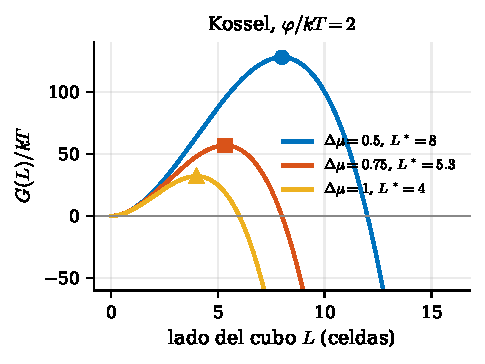
\includegraphics[width=\linewidth]{gibbs_thomson.pdf}\caption{teoría~\eqref{eq:GT}}\end{subfigure}\hfill
\begin{subfigure}[b]{0.57\linewidth}\centering
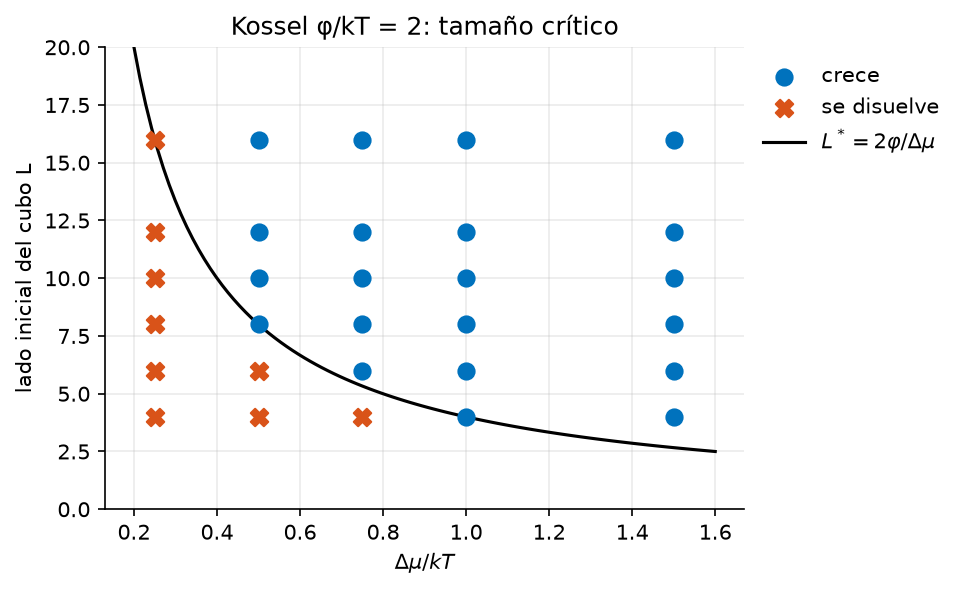
\includegraphics[width=\linewidth]{kossel_tamano_critico.png}\caption{kMC: crece / se disuelve}\end{subfigure}
\caption{Tamaño crítico de un cubo de Kossel ($\varphi/kT=2$). (a) $G(L)$ y su máximo. (b) Resultado
de cada corrida según el lado inicial y $\dmu$, con la curva $L^*=2\varphi/\dmu$ (notebook~01, \S3.1).}
\label{fig:gt}
\end{figure}

\subsection{Kossel: caras lisas frente a rugosas}

En una cara SOS rugosa cada columna tiene un sitio de unión con tasa $k^+$ y el despegue medio iguala al
del kink, $k^+e^{-\dmu}$, de donde la ley de Wilson--Frenkel~\cite{weeks1979}
\begin{equation}
R/k^+=1-e^{-\dmu}\qquad(\text{capas por }1/k^+).
\label{eq:wf}
\end{equation}
Una cara lisa ($\varphi$ por encima de la rugosidad, \S\ref{sec:gasred}) necesita nucleación 2D y
$R\approx0$ a $\dmu$ bajo. La Fig.~\ref{fig:rough} lo reproduce con tasas de Gilmer: con $\varphi=3$ la
$\{100\}$ casi no avanza para $\dmu\le1$ ($R/k^+<0.04$); con $\varphi=1$ avanza desde el $\dmu$ más
bajo. \textbf{El modelo 3D no es SOS}: en una cara rugosa los lados de los salientes también son sitios
de unión y con Gilmer cada uno recibe $k^+$, de modo que $R/k^+$ supera~\eqref{eq:wf} (1.6 frente a 0.63
con $\varphi=1$, $\dmu=1$). No es un error (el estado incremental coincide con la reconstrucción), sino
una propiedad del gas de red 3D. El plano más externo sobrestima $R$ (2.5 frente a 1.65 en el mismo caso).

\begin{figure}[t]
\centering
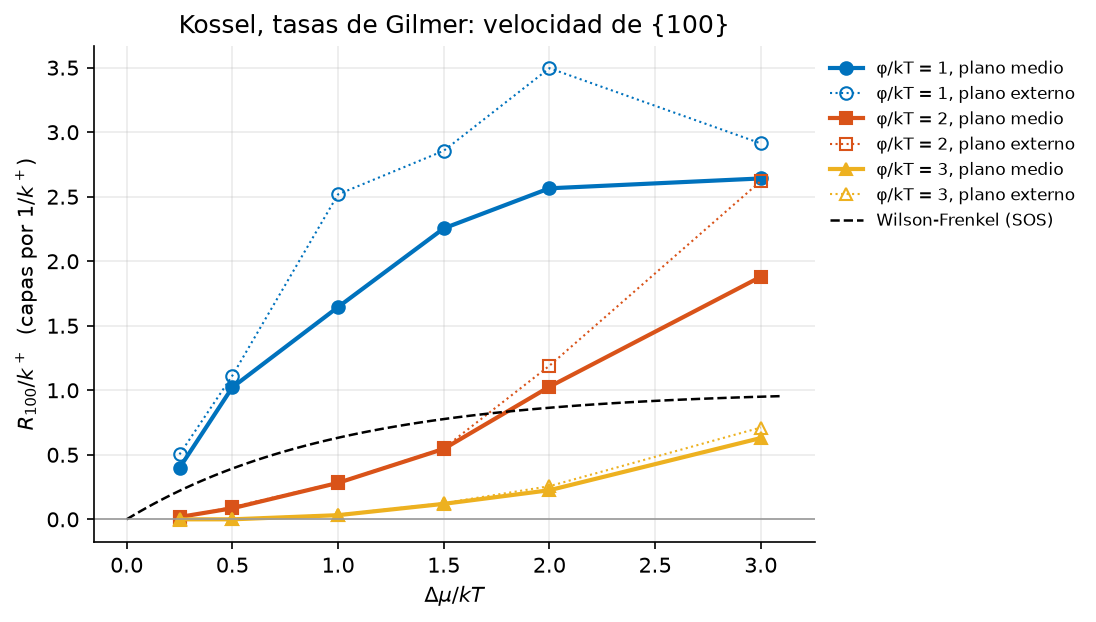
\includegraphics[width=0.72\linewidth]{kossel_R_vs_dmu.png}
\caption{Velocidad de $\{100\}$ en Kossel (Gilmer) frente a $\dmu$ para $\varphi/kT=1,2,3$: plano medio
(continua) y más externo (punteada), con la ley de Wilson--Frenkel SOS (notebook~01, \S3.2).}
\label{fig:rough}
\end{figure}

\subsection{Cubitos anisótropos}

Con $(\varphi_x,\varphi_y,\varphi_z)=(1.2,1.8,3.0)$ cada cara $\{100\}$, $\{010\}$, $\{001\}$ corta un
solo tipo de enlace: $|\Eatt|=\varphi_x,\varphi_y,\varphi_z$, es decir, $1:1.5:2.5$. El kMC (Gilmer,
$\dmu=1$, plano medio) da $R=1:1.66:3.04$ y una aguja según $z$ ($L_1/L_2=1.6$, eje a $2^\circ$ de
$[001]$; Fig.~\ref{fig:aniso}). \textbf{La cinética amplifica la anisotropía} respecto a $\Eatt$ porque
la cara lenta es lisa.

\begin{figure}[t]
\centering
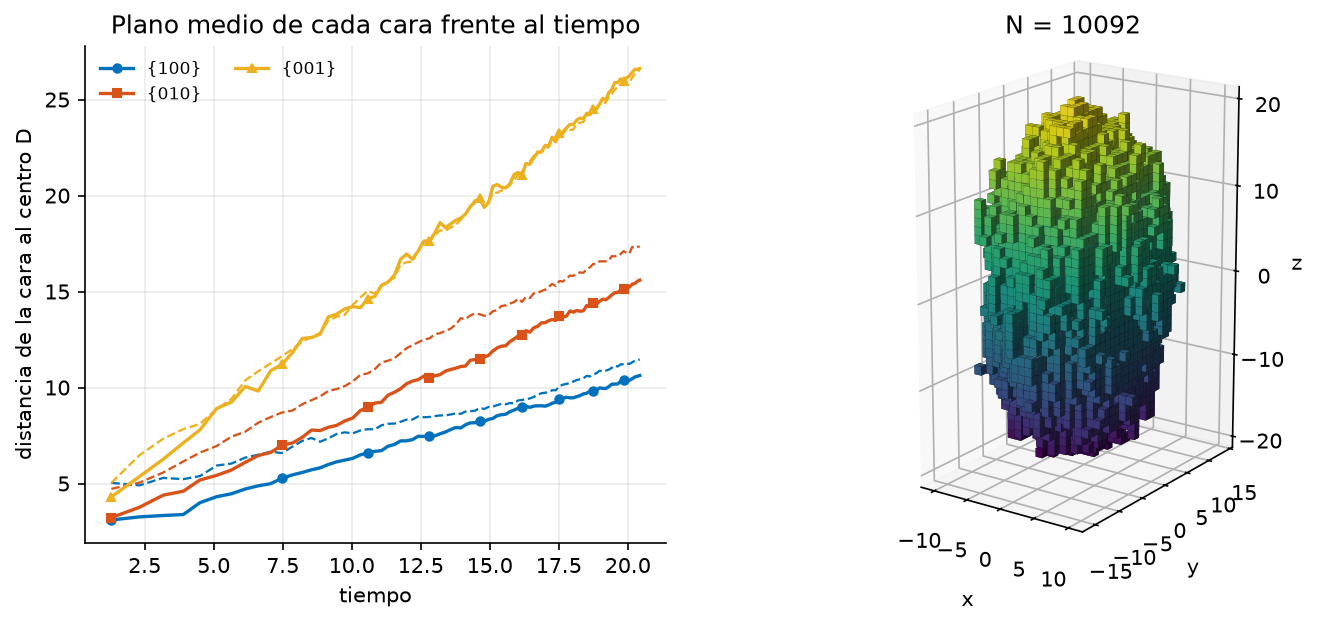
\includegraphics[width=0.86\linewidth]{cubitos_anisotropos.png}
\caption{Cubitos anisótropos (notebook~01, \S4): plano medio de cada cara frente al tiempo
(continua $+$, discontinua $-$) y el cristal a $N\approx10^4$.}
\label{fig:aniso}
\end{figure}

\subsection{\texorpdfstring{$\beta$}{beta}-hematina con energías provisionales}

\paragraph{Forma de energía de unión.} Con~\eqref{eq:ratt} y las caras de la Tabla~\ref{tab:bh}, el
poliedro~\eqref{eq:wulff} es una aguja según $\vect c$: $L_1/L_2=2.05$, $L_2/L_3=1.51$, eje a
$1.8^\circ$ de $[001]$ (Fig.~\ref{fig:bhforma}a).

\paragraph{Barrido en $\dmu$.} Semilla esférica de 70\,Å (unas 870 unidades) hasta $N=40\,000$, con
$\dmu\in\{0.75,1,1.5,2.5\}$ y tasas Gilmer y simétricas. \textbf{El kMC no da la aguja observada}: sale una
lámina poco alargada ($L_1/L_2\approx1.1$--$1.3$, $L_2/L_3\approx2$ a $\dmu\le1$) cuyo eje largo no es $\vect c$: la
dirección de red más próxima es $[001]$ o $[01\bar2]$, a $16$--$21^\circ$. La cinética no sigue a $|\Eatt|$: la $\{010\}$ avanza 2.3--3.6 veces más
rápido que la $\{100\}$ (frente a 1.47) y las caras S $\{110\}$, $\{1\bar10\}$ y la $\{101\}$ son mucho más
lentas de lo predicho, y recortan la aguja (Fig.~\ref{fig:bhR}). Que unas caras S sean lentas va contra
la intuición de Hartman--Perdok; la causa no se ha analizado todavía. \textbf{La anisotropía cae con $\dmu$} (rugosidad cinética; Fig.~\ref{fig:bhshape}a).

\paragraph{Sensibilidad.} La Tabla~\ref{tab:sens} compara tres juegos de energías ($\dmu=1$,
simétricas). Reforzar el apilamiento ($[001]=3.5$) da una aguja según $\vect c$ con $L_1/L_2\approx2$;
escalar además todas las energías $\times1.3$ (bajar la temperatura efectiva) da $L_1/L_2\approx6$
(Fig.~\ref{fig:bhforma}b), pero entonces la (100) casi no crece, el espesor es el de la semilla y la forma
de Wulff cinética es una lámina de espesor casi nulo: \textbf{no es estacionaria}. En los otros dos casos
la forma de Wulff construida con las $R$ medidas reproduce la simulada.

\begin{table}[h]
\centering\small
\caption{Sensibilidad de la forma a las energías de \bh{} ($\dmu=1$, simétricas, $N=40\,000$).}
\label{tab:sens}
\begin{tabular}{@{}lccccccc@{}}
\toprule
& \multicolumn{3}{c}{kMC} & \multicolumn{2}{c}{Wulff cinético ($R$ medidas)} & \multicolumn{2}{c}{$R\propto|\Eatt|$}\\
\cmidrule(lr){2-4}\cmidrule(lr){5-6}\cmidrule(l){7-8}
Energías & $L_1/L_2$ & $L_2/L_3$ & eje & $L_1/L_2$ & $L_2/L_3$ & $L_1/L_2$ & $L_2/L_3$\\
\midrule
provisionales & 1.17 & 1.99 & $[01\bar2]$ & 1.04 & 2.18 & 2.05 & 1.51\\
$[001]=3.5$ & 1.99 & 2.06 & $[001]$ & 2.30 & 2.11 & 2.51 & 1.51\\
$[001]=3.5$, $\times1.3$ & 6.24 & 2.00 & $[001]$ & 8.69 & $\sim1400$ & 2.51 & 1.51\\
\bottomrule
\end{tabular}
\end{table}

\begin{figure}[t]
\centering
\begin{subfigure}[b]{0.36\linewidth}\centering
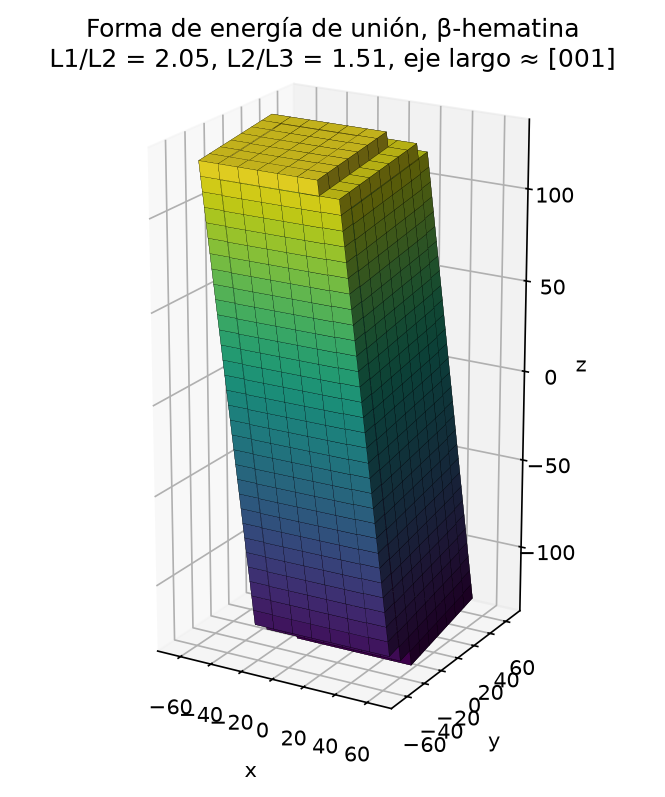
\includegraphics[height=6.0cm]{forma_energia_union_bh.png}\caption{forma de energía de unión}\end{subfigure}\hspace{1cm}
\begin{subfigure}[b]{0.36\linewidth}\centering
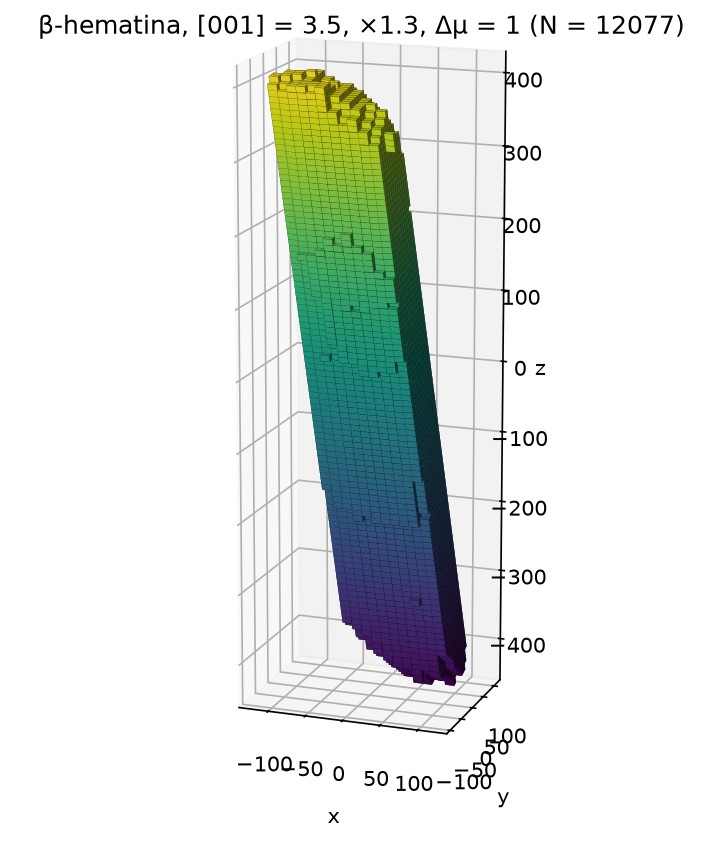
\includegraphics[height=6.0cm]{bh_voxeles.png}\caption{kMC, $[001]=3.5$, $\times1.3$}\end{subfigure}
\caption{\bh{} en vóxeles con la celda triclínica real. (a) Poliedro con $R\propto|\Eatt|$
(energías provisionales). (b) Cristal simulado a $N\approx12\,000$ ($\dmu=1$, simétricas).}
\label{fig:bhforma}
\end{figure}

\begin{figure}[t]
\centering
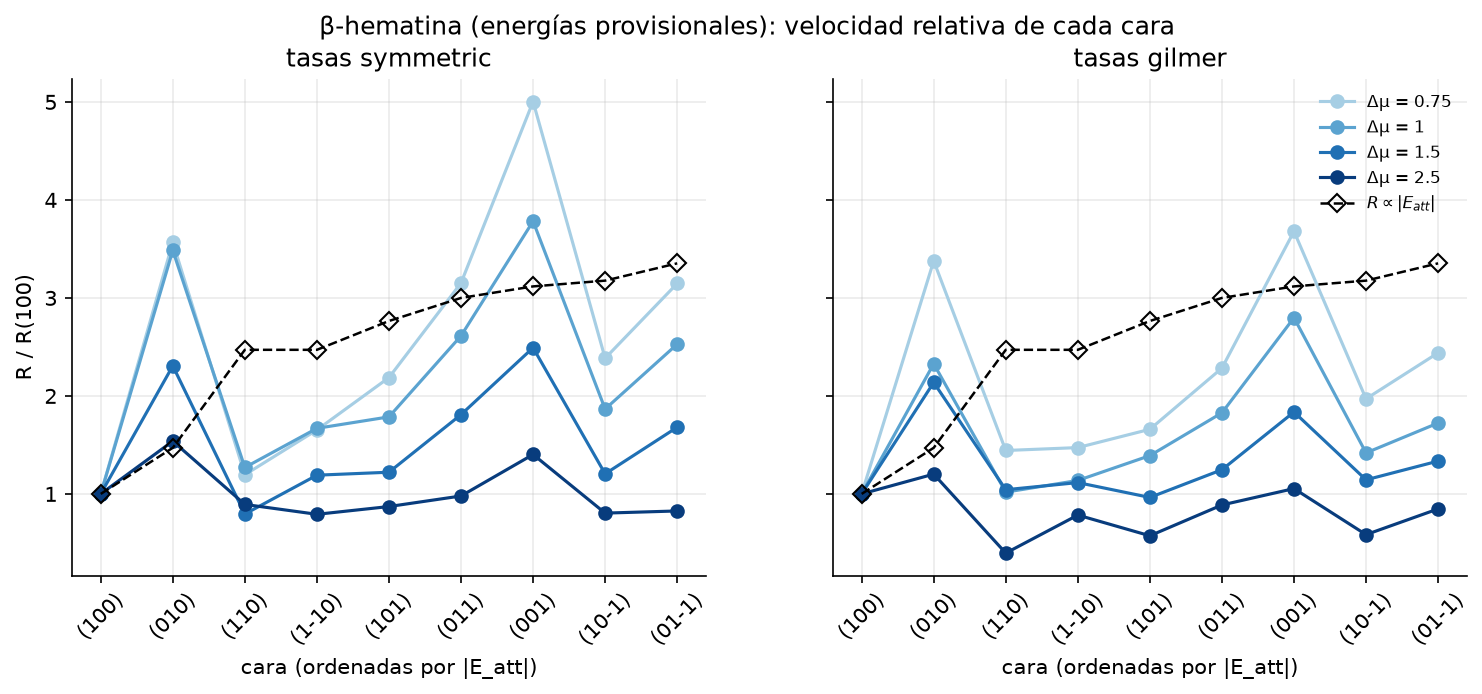
\includegraphics[width=\linewidth]{bh_R_por_cara.png}
\caption{Velocidad de cada cara de \bh{} relativa a la $(100)$, ordenadas por $|\Eatt|$, frente a la
predicción~\eqref{eq:ratt} (rombos), para los dos modelos de tasas y cuatro valores de $\dmu$.}
\label{fig:bhR}
\end{figure}

\begin{figure}[t]
\centering
\begin{subfigure}[b]{0.49\linewidth}\centering
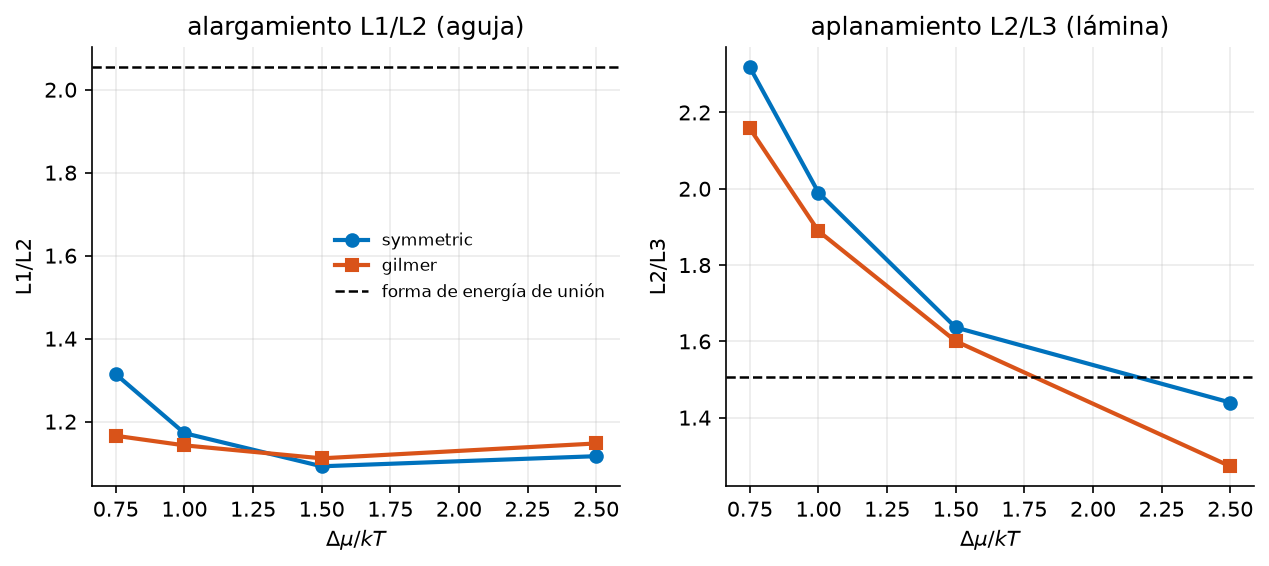
\includegraphics[width=\linewidth]{bh_forma_vs_dmu.png}\caption{forma frente a $\dmu$}\end{subfigure}\hfill
\begin{subfigure}[b]{0.49\linewidth}\centering
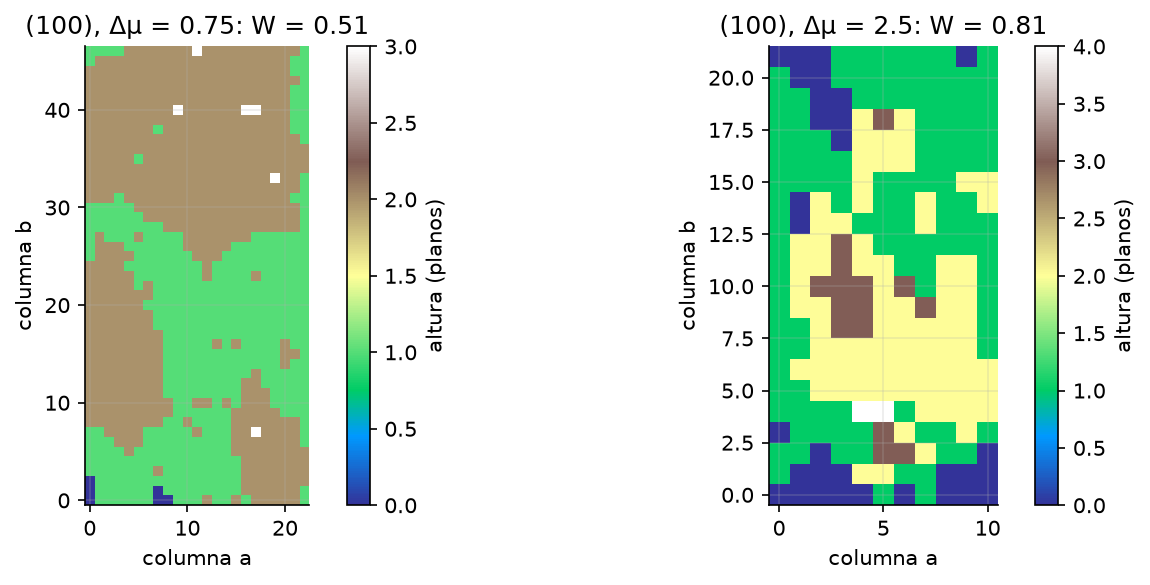
\includegraphics[width=\linewidth]{bh_mapa_alturas_100.png}\caption{mapa de alturas de $(100)$}\end{subfigure}
\caption{(a) Alargamiento y aplanamiento del cristal simulado frente a la forma de energía de unión
(discontinua). (b) Superficie de la $(100)$ (simétricas) analizada con \code{src.analysis}: $W$ pasa de
0.52 a 0.81 y la densidad de escalones de 0.14 a 0.36 entre $\dmu=0.75$ y $2.5$.}
\label{fig:bhshape}
\end{figure}

\paragraph{Probabilidad de unión.} \eqref{eq:Pn} depende mucho del modelo de tasas
(Fig.~\ref{fig:bhP}): con Gilmer solo refleja la abundancia de sitios (los de un vecino son el 20--27\,\%);
con tasas simétricas dominan los sitios muy coordinados (los de 5 o más vecinos suman el 68--77\,\%). La
elección del modelo de tasas (D2) no es un detalle.

\begin{figure}[t]
\centering
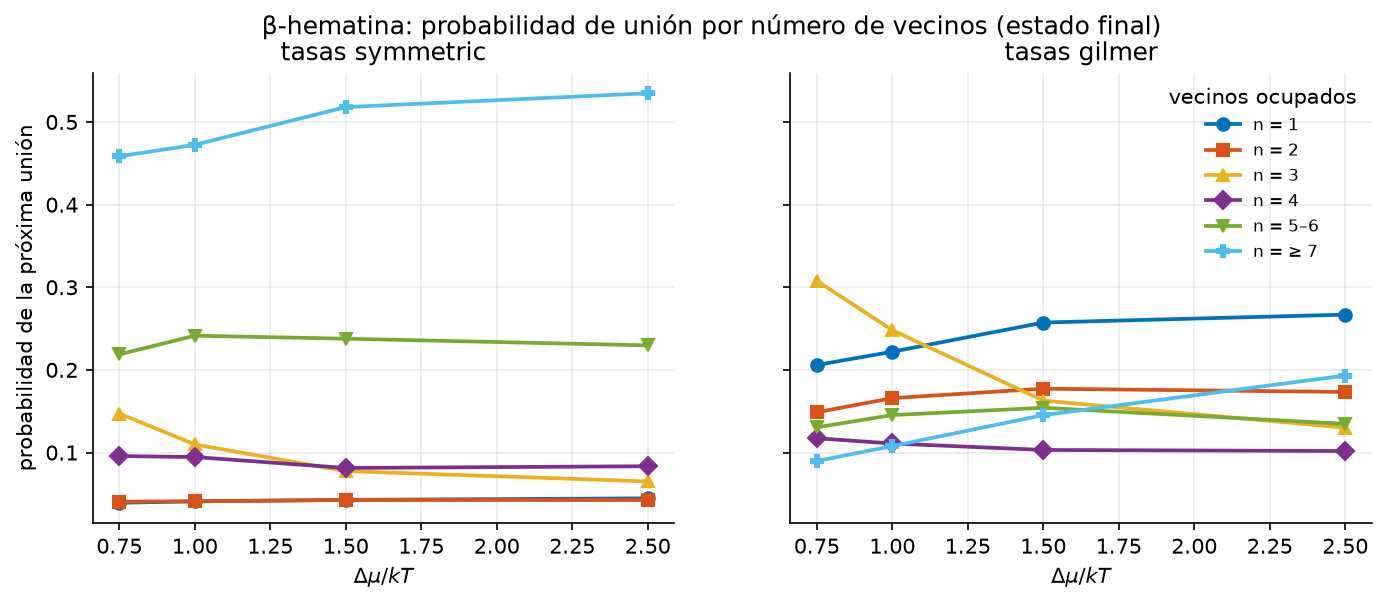
\includegraphics[width=0.85\linewidth]{bh_probabilidad_union.png}
\caption{Probabilidad de que la próxima unión ocurra en un sitio con $n$ vecinos ocupados, en el estado
final de cada corrida del barrido de \bh{} (notebook~01, \S7).}
\label{fig:bhP}
\end{figure}

% =============================================================================
\section{Supuestos, limitaciones y decisiones abiertas}
\label{sec:supuestos}
% =============================================================================

\begin{table}[H]
\centering\small
\caption{Resumen de supuestos. S1--S8 se detallan en el texto; S9--S14 completan la lista.}
\label{tab:supuestos}
\begin{tabularx}{\linewidth}{@{}lY@{}}
\toprule
& Supuesto\\
\midrule
S1 & Red de Bravais con una unidad de crecimiento por celda, sin orientación; dinámica independiente de la métrica.\\
S2 & Energía aditiva por pares, de corto alcance, efectiva en solución ($kT$), sin muchos cuerpos ni elasticidad.\\
S3 & Solución ideal, reservorio infinito, $\dmu$ constante y uniforme; control por superficie.\\
S4 & Kink como referencia: $\mu_{\rm cr}=-\Ecr$; sin entropía vibracional de la unidad.\\
S5 & Tasas de Arrhenius con un único $k_0$; dependencia del sitio solo por $E$; reparto $(a,b)$ fijo.\\
S6 & Solo unión y despegue de una unidad; sin difusión superficial, agregados ni nucleación en solución.\\
S7 & Llegada local (sitios con algún vecino); accesibilidad por sitio; sin vacantes en el volumen.\\
S8 & Análisis: $R\propto|\Eatt|$ solo como referencia; Wulff cinético estacionario; error de borde $O(1/L)$.\\
S9 & Temperatura constante y uniforme, absorbida en las $\varphi_t$ (sin calor latente ni gradientes térmicos).\\
S10 & Sin impurezas, aditivos ni especies adsorbidas (los aditivos son F4).\\
S11 & Cristal perfecto: sin dislocaciones de tornillo, de modo que no hay crecimiento en espiral (BCF~\cite{bcf1951}); una cara lisa solo avanza por nucleación 2D.\\
S12 & Cristal único y aislado: sin otros cristales, sin paredes, sin agregación ni rotura.\\
S13 & Las dos caras $\pm(hkl)$ de una familia son equivalentes (P$\overline1$ centrosimétrico).\\
S14 & Energías de \bh{} provisionales, sin origen físico calculado (D3).\\
\bottomrule
\end{tabularx}
\end{table}

\begin{table}[H]
\centering\small
\caption{Decisiones abiertas para el autor (\code{PLAN\_3DkMC.md}, \S8).}
\label{tab:decisiones}
\begin{tabularx}{\linewidth}{@{}l>{\raggedright\arraybackslash}p{3.3cm}Y>{\raggedright\arraybackslash}p{3.3cm}@{}}
\toprule
& Decisión & Opciones & Por defecto ahora\\
\midrule
D1 & Unidad de \bh{} & dímero (una por celda) / hemo (base 2, F6) & dímero\\
D2 & Modelo de tasas & Gilmer / simétrico / intermedio / adaptativo & Gilmer (Kossel), simétrico (\bh{})\\
D3 & Origen de las energías & campo de fuerzas o DFT / ajuste a morfología y AFM / provisionales & provisionales\\
D4 & ¿Se llenan huecos cerrados? & no (la solución no llega) / sí & no\\
D5 & Fuerza impulsora & $\dmu$ constante / reservorio finito (F4) & constante\\
D6 & Conteo al comparar con 2D & geométrico (3D) / altura exactamente igual (2D) & cada línea con la suya\\
D7 & Escala de tiempo & $k_0=1$ / calibrada con AFM & $k_0=1$\\
D8 & Unidades sueltas & se despegan con su tasa / se eliminan & se despegan\\
\bottomrule
\end{tabularx}
\end{table}

\paragraph{Limitaciones.} (i) \emph{Tamaño}: en Python puro se simulan $10^5$--$10^6$ unidades,
decenas de unidades de lado, lejos de las micras reales; las relaciones de aspecto de un cristal pequeño
están afectadas por aristas y por el tamaño crítico. (ii) \emph{Rugosidad cinética}: a $\dmu$ alto todas
las caras se vuelven rugosas y la anisotropía se comprime; hay que comparar a $\dmu$ experimentales.
(iii) \emph{No es SOS}: más de un sitio de unión por columna en caras rugosas. (iv) \emph{Semilla}: si una
cara casi no crece, su espesor lo fija la semilla y la forma no es estacionaria. (v) Sin difusión
superficial, la cinética de escalones no es la real. (vi) Toda conclusión cuantitativa sobre \bh{} depende
de D3.

\begin{nota}{Observaciones técnicas sobre la implementación}
\begin{enumerate}[leftmargin=*]
\item \textbf{Irreversibilidades locales.} Con \code{allow\_enclosed=True}, llenar un hueco cerrado es
irreversible: la unidad queda con $c=c_{\rm full}$ y no puede despegarse. Igualmente, una unidad suelta
($c=0$) se despega (D8), pero la unión inversa a un sitio sin vecinos está prohibida. En esas transiciones
no hay balance detallado; el resto de la dinámica sí lo cumple (\S\ref{sec:gasred}).
\item \textbf{Cavidades selladas} de más de un sitio sí se llenan (S7): la accesibilidad no se comprueba
por conectividad con el exterior.
\item \textbf{Snapshots por tiempo}: el snapshot de tiempo $t_s$ guarda el estado tras el primer evento con
$t\ge t_s$, que ya incluye ese evento (en BKL el estado en $[t_{\rm old},t_{\rm new})$ es el anterior). La
diferencia es de un evento y es despreciable estadísticamente.
\item \textbf{Coste} $O(T\log K)$ por evento, no $O(T+\log K)$; ver \S\ref{sec:incremental}.
\item \code{viz.plot\_surface\_points} define la superficie con los 6 vecinos de índices, no con los $2T$
del grafo: en \bh{} no coincide con la superficie del motor (\code{KMC3D.surface\_coords}). Solo afecta
al dibujo.
\end{enumerate}
\end{nota}

% =============================================================================
\section{Hoja de ruta}
\label{sec:ruta}
% =============================================================================

\begin{itemize}
\item \textbf{F2, modo \emph{slab}}: caja periódica en las dos direcciones de una cara $(hkl)$ (base de
\code{face\_frame}) y crecimiento solo hacia $+\vect w$. Es el equivalente 3D de MONTY y del motor 2D:
curvas $R_{hkl}(\dmu)$ sin aristas ni tamaño finito, y comparación con \code{KMC\_BKL\_Static} en (001)
con \code{AdaptiveRates} y sin voladizos.
\item \textbf{F3, calibración de \bh{}}: energías de par por campo de fuerzas o DFT, o ajuste a la
morfología (aguja según $\vect c$, $\{100\}$ y $\{010\}$ laterales con anchura/espesor $\approx3{:}1$,
extremos $\{011\}>\{001\}$, sin $\{01\bar1\}$) y a las velocidades AFM de la (100)~\cite{olafson2015},
\emph{usando el kMC}, no solo $\Eatt$: la escala global importa tanto como el reparto.
\item \textbf{F4, física adicional}: difusión superficial (un evento más, con clases código de origen
$\times$ dirección); reservorio finito $\dmu(t)$ sin recalcular todas las clases en cada evento; aditivos
(quinolinas en $\{001\}$, $\{011\}$~\cite{solomonov2007}); tasas adaptativas en 3D.
\item \textbf{F5, rendimiento}: réplicas en paralelo (\code{multiprocessing}); compilar el bucle (numba o
C, ganancia esperada 50--100$\times$; numba no está en las librerías permitidas y necesita el visto bueno
del autor).
\item \textbf{F6, unidades realistas}: base $>1$ (nodos (celda, posición)), criterio F por redes
conexas~\cite{grimbergen1998}, grafo desde un CIF y orientación de la unidad.
\end{itemize}

% =============================================================================
\begin{thebibliography}{99}
\small\setlength{\itemsep}{1pt}
\bibitem{bortz1975} A.\,B. Bortz, M.\,H. Kalos, J.\,L. Lebowitz, \emph{J. Comput. Phys.} \textbf{17}, 10 (1975). Algoritmo \emph{n-fold way}.
\bibitem{fenwick1994} P.\,M. Fenwick, \emph{Softw. Pract. Exper.} \textbf{24}, 327 (1994). Árbol de Fenwick.
\bibitem{gilmer1972} G.\,H. Gilmer, P. Bennema, \emph{J. Appl. Phys.} \textbf{43}, 1347 (1972). kMC de Kossel.
\bibitem{kossel1927} W. Kossel, \emph{Nachr. Ges. Wiss. Göttingen, Math.-Phys. Kl.}, 135 (1927).
\bibitem{stranski1928} I.\,N. Stranski, \emph{Z. Phys. Chem.} \textbf{136}, 259 (1928).
\bibitem{bcf1951} W.\,K. Burton, N. Cabrera, F.\,C. Frank, \emph{Phil. Trans. R. Soc. A} \textbf{243}, 299 (1951).
\bibitem{hartman1955} P. Hartman, W.\,G. Perdok, \emph{Acta Cryst.} \textbf{8}, 49 (1955). Teoría PBC; caras F/S/K.
\bibitem{hartman1980} P. Hartman, P. Bennema, \emph{J. Cryst. Growth} \textbf{49}, 145 (1980). Energía de unión y velocidad de cara.
\bibitem{grimbergen1998} R.\,F.\,P. Grimbergen, H. Meekes, P. Bennema, C.\,S. Strom, L.\,J.\,P. Vogels, \emph{Acta Cryst. A} \textbf{54}, 491 (1998).
\bibitem{frank1958} F.\,C. Frank, en \emph{Growth and Perfection of Crystals}, R.\,H. Doremus et al. (eds.), Wiley (1958), p.~411. Teoría cinemática; forma de Wulff cinética.
\bibitem{weeks1979} J.\,D. Weeks, G.\,H. Gilmer, \emph{Adv. Chem. Phys.} \textbf{40}, 157 (1979). Dinámica de crecimiento, rugosidad, SOS.
\bibitem{hasenbusch1996} M. Hasenbusch, S. Meyer, M. Pütz, \emph{J. Stat. Phys.} \textbf{85}, 383 (1996). Rugosidad de la interfaz de Ising 3D.
\bibitem{boerrigter2004} S.\,X.\,M. Boerrigter et al., \emph{J. Phys. Chem. A} \textbf{108}, 5894 (2004). MONTY.
\bibitem{anderson2017} M.\,W. Anderson et al., \emph{Nature} \textbf{544}, 456 (2017). CrystalGrower.
\bibitem{pagola2000} S. Pagola, P.\,W. Stephens, D.\,S. Bohle, A.\,D. Kosar, S.\,K. Madsen, \emph{Nature} \textbf{404}, 307 (2000). Estructura de \bh{}.
\bibitem{solomonov2007} I. Solomonov et al., \emph{J. Am. Chem. Soc.} \textbf{129}, 2615 (2007). Morfología de \bh{} y quinolinas.
\bibitem{olafson2015} K.\,N. Olafson, M.\,A. Ketchum, J.\,D. Rimer, P.\,G. Vekilov, \emph{PNAS} \textbf{112}, 4946 (2015). Crecimiento por capas de hematina (AFM).
\bibitem{nagpal2024} Nagpal et al. (2024), \code{references/modern\_kMC/}. Tasas adaptativas del modelo 2D.
\end{thebibliography}

\end{document}
